\documentclass[journal]{IEEEtran}

\def\pub{false} % true for publication, false for draft
\newcommand*{\template}{template} 
\input{\template/preamble/preamble_journal.tex}

\newcommand*{\figSizeTwoCol}{.49}
\newcommand*{\figSizeOneCol}{0.98}

\begin{document}

\title{
    Constrained Optimization-Based Neuro-Adaptive Control (CONAC) for Euler-Lagrange Systems Under Weight and Input Constraints
} %% Article title

\author{
  Myeongseok Ryu, Donghwa Hong, and Kyunghwan Choi
\thanks{
    Myeongseok Ryu and Kyunghwan Choi are with the Cho Chun Shik Graduate School of Mobility, Korea Advanced Institute of Science and Technology (KAIST), Daejeon 34051, Korea (e-mail: dding\_98@kaist.ac.kr and kh.choi@kaist.ac.kr).

    Donghwa Hong is with the Department of Mechanical and Robotics Engineering, Gwangju Institute of Science and Technology (GIST), Gwangju 61005, Korea (e-mail: fairytalef00@gm.gist.ac.kr).

    This work was supported in part by a Korea Research Institute for Defense Technology planning and advancement (KRIT) grant funded by Korea government DAPA (Defense Acquisition Program Administration) (No. KRIT-CT-22-087, Synthetic Battlefield Environment based Integrated Combat Training Platform) and in part by the National Research Foundation of Korea (NRF) grant funded by the Korea government (MSIT) (RS-2025- 00554087). (Corresponding author: Kyunghwan Choi)
    }}

\markboth{Journal of \LaTeX\ Class Files,~Vol.~18, No.~9, September~2020}%
{How to Use the IEEEtran \LaTeX \ Templates}

\maketitle

%% Abstract
\begin{abstract}
  This study presents a constrained optimization-based neuro-adaptive control (CONAC) for \color{red}unkown\color{black} Euler-Lagrange systems subject to weight and convex input constraints. 
  A deep neural network (DNN) is employed to approximate the ideal stabilizing control law while simultaneously learning the unknown system dynamics and addressing both types of constraints within a constrained optimization framework.
  The adaptation law of DNN weights is formulated to solve the defined constrained optimization problem, ensuring satisfaction of first-order optimality conditions at steady state.
  The controller's stability is rigorously analyzed using Lyapunov theory, guaranteeing bounded tracking errors and bounded DNN weights. 
  The proposed controller is validated through a real-time implementation on a 2-DOF robotic manipulator, demonstrating its effectiveness in achieving accurate trajectory tracking while satisfying all imposed constraints.
\end{abstract}

\begin{IEEEkeywords}
    Neuro-adaptive control, constrained optimization, deep neural network, input constraint.
\end{IEEEkeywords}

\section*{Notation}
In this study, the following notation is used:

\begin{itemize}
    \item := denotes ``is defined as" or ``is equal to".
    \item $\R$ and $\R^{n\times m}$ denote the set of real numbers and $n\times m$ dimensional matrices, respectively, and $\R_{\ge0}:=[0,\infty)$ and $\R_{>0}:=(0,\infty)$.
    \item $(\cdot)^\top$ denotes the transpose of a vector or matrix.
    \item $\norm{\cdot}$ and $\norm{\cdot}_F$ denote the Euclidean norm and Frobenius norm, respectively.
    \item $\otimes$ denotes the Kronecker product \cite[Chap. 7, Def. 7.1.2]{Bernstein:2009aa}.
    \item A vector and a matrix are denoted by $\mv{x}=[x_i]_{i\in\{1,\cdots,n\}}\in\R^n$ and $
        \mm A
        := 
        [a_{ij}]
        _{
            i\in\{1,\cdots,n\},j\in\{1,\cdots ,m\}
        }\allowbreak\in\R^{n\times m}
        $, respectively.
    \item $\myrow_i(\mm A)$ denotes the $i\textsuperscript{th}$ row of the matrix $\mm A\in\R^{n\times m}$. 
    \item For the matrix $\mm{A}\in\R^{n\times m}$, $\myvec(\mm A):=\left(\myrow_1(\mm A^\top),\cdots,\myrow_m(\mm A^\top) \right)^\top\in\R^{nm}$ denotes the vectorization of $\mm A$.
    % \item $\mycol_i(A)$ and $\myrow_j(A)$ denote the $i\textsuperscript{th}$ column and $j\textsuperscript{th}$ row of $A\in\R^{n\times m}$, respectively.
    % \item $\myvec(A):= [\mycol_1(A)^\top  ,\cdots,\mycol_m(A)^\top  ]^\top   $ for $A\in\R^{n\times m}$.
    \item $\lambda_{\min}(\mm A)$ denotes the minimum eigenvalue of the matrix $\mm A\in\R^{n\times n}$.
    \item $\mm I_n$ denotes the $n\times n$ identity matrix, and $\mm 0_{n\times m}$ denotes the $n\times m$ zero matrix.
\end{itemize}

%  SECTION INTRODUCTION ===================================
\section{Introduction}

\subsection{Background}

\IEEEPARstart{M}{any} engineering systems, including those in aerospace, robotics, and automotive applications, can be modeled using Euler-Lagrange systems. 
These systems are governed by dynamic equations derived from energy principles and describe the motion of mechanical systems with constraints. 
In practice, however, such systems often exhibit uncertainties due to unmodeled dynamics, parameter variations, or external disturbances. 
These uncertainties can significantly degrade control performance and, in some cases, lead to instability. 
To address these challenges, adaptive control methods have been widely employed to ensure robust performance in the presence of system uncertainties \cite{Ioannou:2006aa, Tao:2003aa}.

More recently, neuro-adaptive control approaches have been introduced to approximate unknown system dynamics or entire control laws using neural networks (NNs) \cite{Lewis:1998aa,Farrell:2006aa}. 
NNs are well-known for their universal approximation property, which allows them to approximate any smooth function over a compact set with minimal error. 
Various types of NNs have been utilized in neuro-adaptive control, including simpler architectures like single-hidden layer (SHL) NNs \cite{Lewis:1996aa,Ge:2010aa, Yesildirek:1995aa} and radial basis function (RBF) NNs \cite{Liu:2013ab,Ge:2002aa}, as well as more complex models like deep NNs (DNNs) \cite{Patil:2022aa} and their variations. 
Conventionally, SHL and RBF NNs are often employed to approximate \color{red}unkown\color{black} system dynamics or controllers due to their simplicity \cite{Esfandiari:2014aa,Esfandiari:2015aa,Yesildirek:1995aa,Gao:2006aa}.
However, since DNNs offer greater expressive power, making them more effective for complex system approximations \cite{Rolnick:2018aa}, variations of DNNs, such as long short-term memory (LSTM) networks for time-varying dynamics \cite{Griffis:2023aa}, physics-informed NNs (PINNs) for leveraging physical system knowledge \cite{Hart:2024aa}, and convolutional NNs (CNNs) for learning historical sensor data \cite{Ryu:2024ac}, have further extended the capabilities of neuro-adaptive control systems.

A critical aspect of neuro-adaptive control is the NN weight adaptation law, which governs how NN weights are updated. 
Most studies derived these laws using Lyapunov-based methods, ensuring the boundedness of the tracking error and weight estimation error, thus maintaining system stability under uncertainty.

However, two significant challenges persist in using NNs for adaptive control. 
First, the boundedness of NN weights is not inherently guaranteed, which can result in unbounded outputs. 
When NN outputs are used directly in the control law, this may lead to excessive control inputs, violating input constraints. 
Such constraints are commonly encountered in industrial systems, where actuators are limited by physical and safety requirements in terms of amplitude, rate, or energy \cite{Esfandiari:2021aa}. 
Failing to address these constraints can degrade control performance or even destabilize the system.

Therefore, addressing these two key issues—ensuring weight boundedness and satisfying input constraints—is essential for the reliable design of neuro-adaptive controllers. 
The following section provides a detailed review of existing solutions to these challenges.

\subsection{Literature Review}

\subsubsection{Ensuring Weight Norm Boundedness}

A common challenge in neuro-adaptive control is maintaining the boundedness of the NN weights to ensure stability. 
In many studies, projection operators were employed to enforce upper bounds on the weight norms, ensuring that the weights do not grow unboundedly. 
For example, in \cite{Zhou:2023aa,Griffis:2023aa,Patil:2022aa}, projection operators were used to constrain the weight norms to remain below predetermined constants. 
However, these constants were often selected as large as possible due to the lack of theoretical guarantees regarding the global optimality of the weight values. 
While this approach ensured that the NN remained stable, it did not necessarily result in optimal performance.

In addition to projection operators, some studies utilized modification techniques like $\sigma$-modification \cite{Ge:2002aa} and $\epsilon$-modification \cite{Esfandiari:2015aa,Gao:2006aa}. 
These methods ensured that the NN weights remained within an invariant set by incorporating stabilizing functions into the adaptation law. 
Although these techniques were effective in ensuring boundedness and avoiding weight divergence, they similarly lacked a formal analysis of the optimality of the adapted weights by biasing the adaptation law toward the origin \cite{Ryu:2024aa}.
This leaves room for improvement in terms of performance optimization.

\hfill

\subsubsection{Satisfying Input Constraints}

The second major issue is satisfying input constraints, particularly in systems where actuators are subject to physical limitations. 
% The unpredictable outputs of NNs can sometimes lead to excessively large control inputs, violating these constraints. 
This issue is exacerbated in neuro-adaptive controllers that utilize NNs as additional control inputs to cancel out uncertain (unknown) system dynamics while conventional model-based control methods, \eg feedback linearization and backstepping, are employed. 
In the cases of feedback linearization and backstepping, controllers may produce overly aggressive control inputs, even when the system's natural dynamics are stabilizing, leading to unnecessary saturation of the control inputs \cite{Khalil:2002aa}.
Moreover, if the control inputs are already saturated, the NNs are enforced to compensate for the saturated inputs.
In other words, the conventional methods deteriorates the learning process by sabotaging the NN adaptation law, as the feedback error for learning is no longer directly related to the NNs' output.
Hence, the input constraint should be handled in an unity adaptation framework \MSRY{Start from here!}

To address this early discussed issue, many studies introduced auxiliary systems to handle input constraint in adaptation process. 
These systems mitigated the effects of control input saturation by modifying the control strategy when saturation occurred. 
For instance, in \cite{Esfandiari:2014aa,Karason:1994aa,Esfandiari:2015aa}, auxiliary states were generated whenever input saturation was detected, and these states were incorporated into the adaptation law to adjust the NN weights accordingly. 
This approach helped the controller reduce input saturation by indirectly regulating the auxiliary states.

Alternatively, auxiliary states can also be used as feedback terms in the control law to directly compensate for the effects of input saturation constraints, as demonstrated in \cite{Arefinia:2020aa,He:2016aa,Peng:2020aa}. 
In \cite{Gao:2006aa}, the NN was used to approximate the desired control input, compensating for input saturation. 
However, these approaches typically handle input bound constraints on a per-input basis, \ie applying bounds to each scalar control variable individually, and may not account for more complex, nonlinear constraints, like input norm constraints, which are commonly found in physical systems such as robotic actuators or motor systems.

\hfill

\subsubsection{Limitations of Existing Approaches and Potential of Constrained Optimization}

Although both the existing methods for weight boundedness and input constraints have shown effectiveness, they come with significant limitations. 
Projection operators and modification techniques do not guarantee the optimality of the adapted weights. 
Moreover, auxiliary systems typically handle only simple forms of input constraints, such as individual input bound constraints, limiting their ability to address more complex, nonlinear constraints.

To overcome these limitations, constrained optimization offers a promising approach. 
By formulating the neuro-adaptive control problem as an optimization problem with constraints, it is possible to adapt the NN weights while minimizing an objective function, \eg tracking error, subject to both weight and input constraints. 
Constrained optimization provides a theoretical framework for defining optimality and presents numerical methods for finding solutions that satisfy the constraints \cite{Nocedal:2006aa}.

In existing literature, constrained optimization techniques, such as the Augmented Lagrangian Method (ALM) \cite{Evens:2021aa} and the Alternating Direction Method of Multipliers (ADMM) \cite{Wang:2019aa,Taylor:2016aa}, have been used to train NNs offline. 
These methods impose constraints to address issues like gradient vanishing in backpropagation. 
However, to the best of the authors' knowledge, no prior work has applied constrained optimization to adaptive control systems with real-time weight adaptation. 
This gap suggests that constrained optimization could be key to addressing both weight boundedness and input constraints in a unified, theoretically grounded framework, particularly in real-time neuro-adaptive control.

\subsection{Contributions}

The main contributions of this study are listed as follows:
\begin{itemize}
    \item A constrained optimization-based neuro-adaptive control (CONAC) is proposed, where the control problem is formulated as a constrained optimization problem. In this formulation, weight and convex input constraints are incorporated as inequality constraints, while minimizing a given objective function.
    % \item Any convex input constraints can be applied to the proposed CONAC, including input bound constraints, and norm constraints. Moreover, the proposed CONAC can handle any combination of these constraints, which can be useful in practical applications where multiple constraints need to be satisfied simultaneously.
    % \item Since the proposed CONAC approximate the entire ideal control law with no prior knowledge of the system dynamics, the system identification process can be avoided, which is often difficult and time-consuming to implement in practice. 
    \item The adaptation laws for DNN weights and Lagrange multipliers are systematically derived to solve the defined problem, using constrained optimization theory. These laws guarantee convergence to the first-order optimality conditions, specifically the Karush–Kuhn–Tucker (KKT) conditions, as described in \cite[Chap. 12, Thm. 12.1]{Nocedal:2006aa}.
    \item The proposed CONAC's stability is rigorously analyzed using Lyapunov theory, ensuring that the tracking error and DNN weights remain bounded. This analysis guarantees that the proposed CONAC can achieve stable adaptation online.
    \item The proposed CONAC is implemented in real-time on a 2-DOF robotic manipulator, demonstrating its effectiveness in achieving accurate trajectory tracking while satisfying all imposed constraints. The experimental results validate the theoretical findings and show the practical applicability of the proposed CONAC.
\end{itemize}

\hfill

This study is extended from our preliminary work presented in \cite{Ryu:2024aa} where the inequality constraint for weight norm was imposed on the neuro-adaptive control design to establish the weight boundedness using constrained optimization framework.
Similar to weight constraints in \cite{Ryu:2024aa}, control input constraints are also incorporated into the CONAC framework to address the convex input saturation problem as well.
Furthermore, the applicability of the proposed CONAC is investigated in a real-time implementation on a 2-DOF robotic manipulator; while the referenced work was limited to the numerical simulation.

\subsection{Organization}

The remainder of this paper is organized as follows. 
Section \ref{sec:Problem Formulation} presents the target system and control objective.
Section \ref{sec:ctrl design} introduces the proposed CONAC and the architecture of DNN in the controller. 
In Section \ref{sec:adap_laws}, the adaptation law is developed.
Section \ref{sec:stability} analyzes the stability of the proposed CONAC.
A real-time implementation of the proposed CONAC is presented in Section \ref{sec:sim}, where the proposed CONAC is applied to a 2-DOF robotic manipulator.
Finally, Section \ref{sec:conclusion} concludes the paper and discusses potential future work.
The candidates of convex input constraints are presented in Appendix \ref{sec:appen:cstr}. 

% ====================================
%  SECTION PROBLEM FORMULATION 
% ====================================
\section{Problem Formulation}\label{sec:Problem Formulation}

\subsection{Model Dynamics and Control Objective}

We consider an \color{red}unkown\color{black} Euler-Lagrange system modeled as
\begin{equation}
    \rbM\ddq +\rbVm \dq+ \rbF + \rbG + \rbd
    =
    \mysat(\rbu)
    ,
    \label{eq:sys1}
\end{equation}
where $\q\in \R^n$ denotes the generalized coordinate, $\rbd$ represents the disturbance and $\rbu\in\R^n$ denotes the generalized control input. 
The terms $\rbM:=\rbM(\q)\in\R^{n\times n}$, $\rbVm:=\rbVm(\q,\dq)\in\R^{n\times n}$, $\rbF:=\rbF(\dq)\in\R^{n}$, and $\rbG:=\rbG(\q)\in\R^{n}$ represent the unknown inertia matrix, Coriolis/centripetal matrix, friction vector, and gravity vector, respectively.
The function $\mysat(\cdot):\R^n\to\R^n$ represents the inherent physical limitations of the actuators such that $\norm{\mysat(\rbu)}\le \overline\tau$, where $\overline\tau\in\R_{>0}$ denotes the maximum norm of control input.

In this study, the saturation function $\mysat(\cdot)$ is assumed to be convex, which is practically common in many engineering systems.
This is because, the actuator limits are naturally convex, such as min/max torque limits, and bounds look like a box or ball in the input space.
To account for these limitations, it is essential to incorporate physically motivated constraints into the controller design.
Appendix \ref{sec:appen:cstr} introduces candidate constraints that can be applied to ensure compliance with these physical limitations.

The Euler-Lagrange system \eqref{eq:sys1} satisfies several important physical properties, as presented in \cite[Chap. 3, Tab. 3.2.1]{Lewis:1998aa}. 
The key properties are introduced below:
\begin{prop} 
    The inertia matrix $\rbM$ is symmetric, positive definite, and bounded.
    \label{prop:M}
\end{prop}

\begin{prop} 
    The Coriolis/centripetal matrix $\rbVm$ can always be selected, so that the matrix $\ddtt{\rbM}-2\rbVm$ is skew-symmetric, \ie $\mv{x}^\top(\ddtt{\rbM}-2\rbVm)\mv{x}=0,\ \forall \mv{x}\in\R^n$.
    \label{prop:skew}
\end{prop}

\begin{prop}
    The disturbance $\rbd$ is bounded, \ie $\norm{\rbd}\le \overline\tau_d$, where $\overline\tau_d\in\R_{\ge0}$.
    \label{prop:dis_bound}
\end{prop}

The control objective is to develop a neuro-adaptive controller that enables $\q$ to track a continuously differentiable desired trajectory $\qd:=\qd(t): \R_{\ge0} \to \R^n$, compensating for the unknown system dynamics while addressing the imposed constraints.
The desired trajectory $\qd(t)$ is supposed to satisfy the following assumption:
\begin{assum}
    The desired trajectory $\qd(t)$ is assumed to be bounded, \ie $\norm{\qd(t)}\le \overline{q}_d\in\R_{>0}$ , and available for designing a bounded control input.
    \label{assum:feasible}
\end{assum}

%  SECTION CONTROLLER DESIGN ==============================
\section{Control Law Development}\label{sec:ctrl design}

The architecture of the proposed CONAC consists of a DNN that functions as a neuro-adaptive controller, and a weight optimizer for the DNN, as illustrated in Fig. \ref{fig:ctrl:diagram}.
The algorithm of the proposed CONAC is given by Algorithm \ref{alg:CONAC}. 
Before proceeding to the controller design, some mathematical preliminaries are revisited in Section \ref{sec:sub:math preliminaries}. 
Section \ref{sec:sub:NAC} introduces the neuro-adaptive controller, followed by the DNN model in Section \ref{sec:sub:NN definition}. 
The constrained optimization-based weight adaptation law is presented in Section \ref{sec:adap_laws}.

\begin{figure}[!t]
    \centering
    \includegraphics[width=.999\linewidth]{src/figures/Controller.drawio.pdf}
    % \includesvg[width=0.75\linewidth]{Controller.drawio.svg}
    \caption{Architecture of the proposed constrained optimization-based neuro-adaptive controller (CONAC).}
    \label{fig:ctrl:diagram}
\end{figure}

\begin{algorithm}[!t]
    \caption{Proposed CONAC Algorithm}\label{alg:CONAC}
    \begin{algorithmic}[1]
        \STATE \textbf{Initialize:} DNN weights $\estwth$ and Lagrange multipliers $\lambda_j$
        \FOR{each sampling time}
            \STATE Measure current state $\q,\dq$
            \STATE Compute filtered error $\fe$ \eqref{eq:err:filtered}
            \STATE Update DNN weights $\estwth$ using $\fe$ \eqref{eq:adap:th}
            \STATE Update Lagrange multipliers $\lambda_j$ based on constraint function $c_j$ \eqref{eq:adap:lbd} and \eqref{eq:adap:lbd:max}
            \STATE Compute control input $\rbu$ (DNN output) \eqref{eq:control:est} and \eqref{eq:DNN:architecture}
            \STATE Apply control input $\rbu$ to the system \eqref{eq:sys1}
        \ENDFOR
    \end{algorithmic}
\end{algorithm}

\subsection{Mathematical Preliminaries}\label{sec:sub:math preliminaries}

The following proposition and lemma will be used in subsequent sections:

\begin{propsit}[see {\cite[Chap. 7, Prop. 7.1.9]{Bernstein:2009aa}}] \label{propsit:kron}
	For a matrix $\mm A\in\R^{n\times m}$ and a vector $\mv b\in\mathbb R^n$, the following property holds:
	\begin{equation}
		\mm A^\top \mv b 
		= 
		\myvec(\mm A^\top\mv b)
		=
		\myvec(\mv b^\top\mm A)
		= 
		(\mm{I}_{m}\otimes \mv b^\top) \myvec(\mm A)
		.
	\end{equation}
\end{propsit}


\begin{lem} \label{lem:stable:set}
    For a Lyapunov function $V:=V(\mv{x})\ge0$ with $\mv{x}\in\R^n$, if the time derivative of $V$ is given by $\ddtt V\le -a_1 \mv{x}^\top \mv{x} + a_2 \mv{x}$ for some positive constants $a_1\in\R_{>0}$ and $a_2\in\R_{>0}$, then $\mv{x}$ is bounded as $\mv{x}\in\{\mv{x}\mid\norm{\mv{x}}\le\tfrac{a_2}{a_1}\}$.
\end{lem}

\begin{proof}
    The time derivative of $V$ can be rewritten as
    \begin{equation}
        \ddtt V
        \le
        -a_1 \norm{\mv{x}}^2 + a_2 \norm{\mv{x}}
        =
        -a_1
        \left(
            \norm{\mv{x}}-\tfrac{a_2}{2a_1}
        \right)^2
        +
        \tfrac{a_2^2}{4a_1}
        .
        \label{eq:lem:lya:dot}
    \end{equation}
    According to \eqref{eq:lem:lya:dot}, one can conclude that $\ddtt V$ is negative definite if $\norm{\mv{x}}>\tfrac{a_2}{a_1}$ holds.
    In other words, $\mv{x}$ remains within the bounded set $\{\mv{x}\mid\norm{\mv{x}}\le\tfrac{a_2}{a_1}\}$, since $\ddtt V$ is negative definite when $\mv{x}$ is outside the set.
\end{proof}


\subsection{Neuro-Adaptive Controller Design}\label{sec:sub:NAC}

Given that the Euler-Lagrange system \eqref{eq:sys1} exhibits second-order dynamics, a filtered error $\fe\in\R^n$ is introduced to convert the system into a first-order system, as follows:
\begin{equation}
    \fe := \ddtt{\mv e}+\mm\Lambda \mv e
    ,
    \label{eq:err:filtered}
\end{equation}
where $\mv e := \q - \qd$ denotes the tracking error, $\ddtt{\mv e} := \dq - \dqd$ represents the time derivative of the tracking error, and $\mm\Lambda\in\R^{n\times n}_{>0}$ is a user-designed filtering matrix.
Since \eqref{eq:err:filtered} is stable system, it implies that $\mv e$ is bounded if $\fe$ is bounded.

Using $\fe$, the system dynamics \eqref{eq:sys1} can be rewritten as
\begin{equation}
   \rbM \ddtt\fe
    =
    -\rbVm \fe
    -\mm K \fe
    + \mv f
    -\rbd + \mysat(\rbu)
    ,
    \label{eq:sys:filtered}
\end{equation}
where $\mm{K}=\mm{K}^\top\in\R^{n\times n}_{>0}$ denotes an arbitrary unknown matrix and $
    \mv f:= \mv f
    \left(
        \q,\dq,\qd,\dqd,\ddqd
    \right)
    =
    \mm K \fe
    +\rbM
    \left(
        -\ddqd+\mm\Lambda\ddtt{\mv e}
    \right)
    +
    \rbVm
    \left(
        -\dqd+\mm\Lambda\mv e
    \right)
    -
    \rbF
    -
    \rbG
    \in\R^n
$ denotes the lumped system uncertainty.
% \color{red}
% The unknown matrix $\mm{K}$ is not available to design in practice, 
% \color{black}

Consider the Lyapunov function $V_1:= \tfrac{1}{2}\fe^\top \rbM\fe$. 
Invoking Property \ref{prop:skew}, the time derivative of $V_1$ is
\begin{equation}
    \begin{aligned}
        \ddtt{V}_1
        =&
        \fe^\top \rbM \ddtt \fe
        +
        \tfrac{1}{2}\fe^\top \ddtt{\rbM}\fe
        \\
        =&
        \fe^\top 
        \left(
            -\rbVm \fe -\mm K \fe + \mv f
            -\rbd + \mysat(\rbu)
        \right)
        \\
        &
        +
        \tfrac{1}{2}
        \fe^\top \ddtt{\rbM}\fe
        \\
        =&
        -
        \fe^\top \mm K \fe 
        +
        \fe^\top 
        \left(
            \mv f
            -\rbd
            +\mysat(\rbu)
        \right)
        \\
        &
        +
        \tfrac{1}{2}
        \fe^\top(\ddtt{\rbM}- 2\rbVm)\fe
        \\
        \le&
        -\lambda_{\min}(\mm K)\norm{\fe}^2
        +
        \overline\tau_d\norm{\fe}
        +
        \fe^\top (\mv f+\mysat(\rbu))
        % \\
        % \le&
        % -\lambda_{\min}(\mm K)\norm{\fe}^2
        % +
        % \overline\tau_d\norm{\fe}
        % +
        % \fe^\top (\mysat(\rbu)-\rbu^*)
        .
    \end{aligned}
    \label{eq:lya1:dot1}
\end{equation} 
Therefore, invoking Lemma \ref{lem:stable:set}, it can be concluded that the filtered error $\fe$ is exponentially stable, with $\lim_{t\to\infty}\norm{\fe}\le\tfrac{\overline\tau_d}{\lambda_{\min}(\mm K)}$, provided that the lumped system uncertainty $\mv{f}$ can be perfectly cancelled by the control input $\rbu$, neglecting the effect of input saturation.
Hence, the ideal control input $\rbu^*$ can be designed as $-\mv f$.
However, $\rbu^*$ is not available in practice, since system dynamics encapsulated in $\mv f$ are unknown.

To overcome this issue, a DNN is employed to approximate $\rbu^*$.
Let $\NN:=\NN({\q}_n;\wth): \R^{l_0+1}\times\R^{\Xi}\to\R^{n}$ represent the DNN, where ${\q}_n\in\R^{l_0+1}$ is the DNN input vector, and $\wth\in\R^{\Xi}$ is the vector of trainable weights.
The architecture of DNN $\NN({\q}_n;\wth)$ will be presented in Section \ref{sec:sub:NN definition}, later.
According to the universal approximation theorem for DNNs \cite{Kidger:2020aa}, $\NN({\q}_n;\wth)$ can approximate a nonlinear function, denoted as $\mv g(\cdot)$, with an ideal weight vector $\idealwth\in\R^\Xi$ over a compact subset $\Omega_{n}\in\R^{l_0+1}$ to within $\epsilon$-accuracy, such that $\sup_{{\q}_n\in\Omega_{n}}\norm{ \NN({\q}_n;\idealwth) - \mv g(\cdot)} = \epsilon < \infty$.
% Furthermore, the theorem states that the norm of $\idealwth$ is bounded such that $\norm{\idealwth}\le \overline\wth<\infty$.
In this study, the ideal weight vector $\idealwth$ is assumed to be bounded by Assumption \ref{assum:feasible} and \cite[Assum. 1]{Lewis:1996aa}, and considered a locally optimal solution, rather than a global one.

Accordingly, the ideal control input $\rbu^*$ can be approximated by the DNN with the ideal weight vector $\idealNN:=\NN({\q}_n;\idealwth)$ as follows:
\begin{align}
    \rbu^*=& \idealNN+\mv\epsilon
    ,
    \label{eq:control:ideal}
\end{align}
where $\mv\epsilon\in\R^n$ is the approximation error vector, bounded by $\norm{\mv\epsilon}\le \overline{\epsilon}$ for some $\overline{\epsilon}\in\R_{>0}$.
The ideal control input $\rbu^*$ is estimated online by
\begin{align}
    \rbu =& \estNN,
    \label{eq:control:est}
\end{align}
where $\hat\NN:=\NN({\q}_n;\estwth)$, and $\estwth\in\R^\Xi$ is the estimated weight vector for the ideal weight vector $\idealwth$.

Substituting \eqref{eq:control:ideal} and \eqref{eq:control:est} into \eqref{eq:lya1:dot1}, the time derivative of $V_1$ can be rewritten as
\begin{equation}
    \ddtt{V}_1
    \le 
    -\lambda_{\min}(\mm K)\norm{\fe}^2
    +
    \overline\tau_d\norm{\fe}
    +
    \fe^\top 
    \left(
        -\idealNN
        -\mv\epsilon
        +\mysat(\hat\NN)
    \right)
    .
    \label{eq:lya1:dot2}
\end{equation}
Therefore, one can conclude that the result of \eqref{eq:lya1:dot1} can be obtained by adapting $\estwth$ to $\idealwth$, \ie $\hat\NN\to\idealNN$, neglecting the effect of input saturation.
Note that the control input saturation has not yet been considered in the derivation of the ideal control input; this will be addressed in the subsequent section.

\subsection{Deep Neural Network (DNN) Model}\label{sec:sub:NN definition}

\begin{figure}[t]
    \centering
    \includegraphics[width=0.99\linewidth]{src/figures/DNN.drawio.pdf}
    \caption{
        Architecture of the DNN $\NN({\q}_n;\wth)$ with $k=2,l_0=2,l_1=l_2=3$, and $l_3=2$.
    }
    \label{fig:DNN}
\end{figure}

The DNN architecture $\NN({\q}_n;\wth) := \NN_k$ can be recursively represented from the $0\textsuperscript{th}$ input layer to the $k\textsuperscript{th}$ output layer, as follows:
\begin{equation}
    \NN_i :=
    \begin{cases}
        \wV_i^\top \act_i(\NN_{i-1}), 
        &
        i\in\{1,\dots ,k\},
        \\
        \wV_0^\top {\q}_n,
        &
        i=0
        ,
    \end{cases}
    \label{eq:DNN:architecture}
\end{equation}
where $\wV_i=[w_{ij}]_{i\in\{1,\cdots,l_i+1\},j\in\{1,\cdots,l_{i+1}\}}\in\R^{(l_i+1)\times l_{i+1}}$ and $\act_i: \R^{l_i}\to\R^{l_i+1}$ represent the weight matrix and the activation function of the $i\textsuperscript{th}$ layer, respectively.
The DNN $\NN({\q}_n;\wth)$ has $k+1$ layers, where the input layer is indexed by $i=0$, and the output layer is indexed by $i=k$.
For instance, in Fig.~\ref{fig:DNN}, the DNN $\NN({\q}_n;\wth)$ with $k=2,l_0=2,l_1=l_2=3$, and $l_3=2$ is illustrated.
Notice that the output size of $\NN(\cdot)$ is the same as that of the control input $\rbu$, \ie $l_{k+1}=n$. 
The weights $\wV_i,\forall i\in\{0,\cdots,k\}$ are initialized randomly using uniform distribution at the beginning of the control process.

The activation function is defined as $\act_i(\mv x):=\left(\sigma(x_1),\sigma(x_2),\cdots, \sigma(x_{l_{i}}), 1\right)^\top,\ \forall\mv x\in\R^{l_i}$, where $\sigma: \R\to\R$ is a nonlinear function, and the augmentation of $1$ is used to account for bias terms in the weight matrices. 
In selecting the nonlinear function $\sigma(\cdot)$, the ReLU function \cite{Maas:2013aa} is one of the widely used functions for large DNNs, since it effectively avoids the gradient vanishing problem during error backpropagation. 
However, for control applications, where relatively shallow DNNs are typically sufficient, and the gradient vanishing issue is less severe, the sigmoid function or the hyperbolic tangent function is commonly used as the nonlinear function $\sigma(\cdot)$. 
These functions simplify stability analysis, since they are continuously differentiable and their outputs and gradients are bounded. 
In this study, the hyperbolic tangent function $\tanh(\cdot)$ was selected as the nonlinear function, \ie $\sigma(x) = \tanh(x),\ \forall x\in\R$, which provides desirable boundedness with $\norm{\sigma(x)}<1$ and $\norm{\ddtfrac{\sigma(x)}{x}}\le 1$.

For simplicity, each layer's weights are vectorized as $\wth_i:=\myvec(\wV_i)\in\R^{\Xi_i},\forall i\in\{0,\cdots,k\}$, where $\Xi_i:= (l_i+1)l_{i+1}$ is the number of weights in the $i\textsuperscript{th}$ layer. 
The total weight vector $\wth\in\R^{\Xi}$ is defined by augmenting $\wth_i, \forall i\in \{0,\cdots,k\}$ as 
\begin{equation}
    \wth := 
    \begin{pmatrix}
        \wth_k\\
        \wth_{k-1}\\
        \vdots\\
        \wth_0
    \end{pmatrix}
    =
    \begin{pmatrix}
        \myvec(\wV_k)\\
        \myvec(\wV_{k-1})\\
        \vdots\\
        \myvec(\wV_0)
    \end{pmatrix},
\end{equation}
where $\Xi={\sum_{i=0}^{k} \Xi_i}$ represents the total number of weights in the DNN.

The gradient of $ \NN({\q}_n;\wth)$ with respect to $\wth$ can be obtained using Proposition \ref{propsit:kron} and the chain rule as follows:
\begin{equation}
    \pptfrac{\NN}{\wth}=
    \begin{bmatrix}
        \pptfrac{\NN}{\wth_k}&
        \pptfrac{\NN}{\wth_{k-1}}&
    \cdots &
        \pptfrac{\NN}{\wth_0}
    \end{bmatrix}
    \in\R^{n \times \Xi}
    ,
    \label{eq:gradient:phi}
\end{equation}
where
\begin{equation}
    \pptfrac{\NN}{\wth_i} = 
    \begin{cases}
        (
            \mm I_{l_{k+1}}
            \otimes 
            \act_{k}^\top  
        )
        , 
        &
        i=k
        ,
        \\
        \wV_k^\top\act_{k}' 
        (
            \mm I_{l_{k}}
            \otimes  
            \act_{k-1}^\top  
        )
        , 
        & 
        i=k-1
        ,
        \\
        &
        \vdots 
        \\
        \wV_k^\top\act'_{k} 
        \cdots 
        \wV_1^\top\act_1' 
        (
            \mm I_{l_1}
            \otimes 
            {\q}_n^\top  
        )
        , 
        &
        i = 0
        ,
    \end{cases}
    \label{eq:NN:grad}
\end{equation}
and $\act_i:= \act_i(\NN_{i-1})$ and $\act_i':= \ddtfrac{\act_i}{\NN_{i-1}}$.

In the following sections, let $\idealNN_i$ represent the output of the $i\textsuperscript{th}$ layer with the ideal weight vector $\idealwth$. 
Additionally, let us define $\idealact_i:=\act_i(\idealNN_{i-1})$ and ${\idealact}'_i:= \ddtfrac{\idealact_i}{\idealNN_{i-1}}$. 
Similarly, $\estNN_i$ denotes the output of the $i\textsuperscript{th}$ layer with the estimated weight vector $\estwth$, and $\estact_i:=\act_i(\estNN_{i-1})$ and $\estact_i':= \ddtfrac{\estact_i}{\estNN_{i-1}}$.

%  SECTION ADAPTATION LAW DERIVATION =======================
\section{Weight Adaptation Laws}\label{sec:adap_laws}

% \subsection{Adaptation Law using Lagrangian Function}
\subsection{Weight Optimizer Design}\label{sec:sub:weight optimizer}

The control objective can be represented as follows:
\begin{equation}
    \begin{matrix}
        \min_{\estwth} \ J(\fe;\estwth):= 
        \tfrac{1}{2} \fe^\top \fe
        ,
        \\ \\
        \begin{aligned}
        \text{subject to }&c_{j}(\estwth) 
        \le0, \quad \forall j\in\mathcal{I},
        \end{aligned}
    \end{matrix}
    \label{eq:opt:problem1}
\end{equation}
where $J(\fe;\estwth)$ is the objective function.
Inequality constraints $c_j:=c_j(\estwth),\ \forall j\in\mathcal{I}$, are imposed during the weight adaptation process to minimize the objective function, where $\mathcal I$ denotes the set of the imposed inequality constraints. 
% Here, $\fe$ is considered a pre-defined data or static parameter for this optimization problem, so that the adaptation process does not consider the dynamics of $\fe$.
The Lagrangian function is defined as
\begin{equation}
    L(
        \fe,\estwth,[\lambda_j]_{j\in\mathcal I}
    ) 
    := 
    J(\fe;\estwth) 
    + 
    \textstyle\sum_{j\in\mathcal I}
    \lambda_{j}
    c_{j}(\estwth)
    ,
    \label{eq:lagrangian}
\end{equation}
where $\lambda_j,\forall j\in\mathcal{I}$ denotes the Lagrange multiplier for each constraint.

The adaptation laws for $\estwth$ and $[\lambda_j]_{j\in\mathcal I}$ are derived to solve the dual problem of \eqref{eq:opt:problem1}, \ie $\min_{\estwth} \max_{[\lambda_j]_{j\in\mathcal I}}L(\fe,\estwth,[\lambda_j]_{j\in\mathcal I})$, as follows:
\begin{subequations}
    \begin{align}
            \ddtt{\estwth}
            &
            =
            -\alpha \pptfrac{L}{\estwth}
            =
            -\alpha 
            \left(
                \pptfrac{J}{\estwth}
                +
                \textstyle\sum_{j\in\mathcal{I}}
                \lambda_j 
                \pptfrac{c_j}{\estwth}
            \right),
        \label{eq:adap:th}
            \\
            \ddtt\lambda_j
            & 
            = 
            \beta_j\pptfrac{L}{\lambda_j} 
            = 
            \beta_j c_j ,
            \quad \forall j\in\mathcal I,
        \label{eq:adap:lbd}
            \\
            \lambda_j & \leftarrow \max(\lambda_j,0) ,
        \label{eq:adap:lbd:max}
    \end{align}
    \label{eq:adaptation law}%             %%
\end{subequations}
where $\alpha\in\R_{>0}$ denotes the adaptation gain (learning rate) and $\beta_j\in\R_{>0}$ denotes the update rate of the Lagrange multipliers in $\mathcal I$, and the arguments of $L(\cdot)$ and $J(\cdot)$ are suppressed for brevity. 
The Lagrange multipliers associated with inequality constraints are non-negative, \ie $\lambda_j\ge 0$, due to \eqref{eq:adap:lbd:max}. 
When a constraint $c_j$ becomes active, \ie $c_j > 0$, the corresponding Lagrange multiplier $\lambda_j$ increases to address the violation, \ie see \eqref{eq:adap:lbd}.
Once the violation is resolved and the constraint is no longer active, \ie $c_j \le 0$, the Lagrange multiplier $\lambda_j$ decreases gradually until it returns to zero.
Note that this adaption law is similar to the ALM in \cite{Nocedal:2006aa}, where the adaptation law for Lagrange multipliers is given by $\lambda_j\leftarrow \max\left(\lambda_j+\tfrac{c_j}{\mu},0\right)$, with $\mu\in\R_{>0}$ being the penalty parameter. 

At steady state, where $\ddtt{\estwth}=0$ and $\ddtt\lambda_j=0$, the KKT conditions are satisfied, \ie $\pptfrac{L}{\estwth}=0$, $c_j \le 0$, $\lambda_j \ge 0$, and $\lambda_j c_j=0$.
In other words, the proposed weight optimizer updates $\estwth$ and $\lambda_j$ in a way that satisfies the KKT conditions. 
These conditions represent the first-order necessary conditions for optimality, guiding the updates toward candidates for a locally optimal point.
% The KKT condition is satisfied, when $\estwth$ converges to $\idealwth$, since $\partial L/\partial \estwth=0$ (i.e. the first-order necessary condition of the optimality is satisfied.).

\subsection{Approximation of the Gradient of Objective Function}

The adaptation law for $\estwth$ defined in \eqref{eq:adap:th} involves the partial derivative of the filtered error with respect to control input $\pptfrac{\fe}{\rbu}$, \ie 
$
    \pptfrac{J}{\rbu}
    =
    \left(
        (\pptfrac{\fe}{\rbu})
        (\pptfrac{\rbu}{\estwth})
    \right)
    ^\top \fe
    =
    \left(
        (\pptfrac{\fe}{\rbu})
        (\pptfrac{\estNN}{\estwth})
    \right)
    ^\top \fe
$. 
Since the objective function depends on $\fe$ of a dynamic system, obtaining $\pptfrac{\fe}{\rbu}$ is not straightforward. 
The recommended method to calculate the exact value of $\pptfrac{\fe}{\rbu}$ is to use the forward sensitivity method \cite{Sengupta:2014aa} by simulating the sensitivity equation as follows: 
\begin{equation}
    \ddtt 
    \left(
        \pptfrac{\fe}{\rbu}
    \right)
    =
    \pptfrac{}{
        \rbu
    }
    \left(
        \rbM^{-1}(
            -\rbVm \fe
            -\mm K \fe
            + \mv f
            -\rbd + \mysat(\rbu)
        )
    \right)
    .
\end{equation}
However, this method cannot be realized, since we do not have the exact system dynamics, \ie $\rbM,\rbVm, \rbF$ and $ \rbG$.
Additionally, the computational cost of the forward sensitivity method is high, as the number of DNN's weights is generally large.

In \cite{Douratsos:2007aa,Saerens:1991aa}, the authors approximate $\pptfrac{\fe}{\rbu}$ by taking the sign of each entry, \ie
$
    \pptfrac{\fe}{\rbu}
    \approx
    \left[
        \mysign(\pptfrac{r_i}{\tau_j})
    \right]_{i,j\in\{1,\cdots,m\}}
$ 
assuming known control directions.
However, this approach is not applicable to \eqref{eq:sys:filtered}, where control directions are unknown.
Instead, since the sign of the control input matrix is known—owing to the positive definiteness of $\rbM^{-1}$, see Property \ref{prop:M}—we approximate $\pptfrac{\fe}{\rbu}\approx \mm I_n$.
Consequently, the adaptation law in \eqref{eq:adap:th} becomes:
\begin{equation}
    \ddtt{\estwth}
    \approx
    -\alpha 
    \left(
        \pptfrac{\estNN}
        {\estwth}^\top
        \fe
        +
        \textstyle\sum_{j\in\mathcal{I}}
        \lambda_j 
        \pptfrac{c_j}{\estwth}
    \right)
    .
    \label{eq:adap:th:approx}
\end{equation}

\subsection{Essential and Potential Constraint Candidates}\label{sec:sub:cstr} 

This section introduces essential constraints required to ensure the stability of the proposed CONAC, as well as conditions for potential control input constraints.

First, weight norm constraints $\mv{c}_{\theta}(\estwth):= [c_{\theta_i}(\estwth)]_{i\in\{0,\cdots ,k\}}\in\mathbb R^{k+1}$ defined in \eqref{eq:cstr:weight:ball}, are essential to prevent the weights from diverging during the adaptation process.
\begin{equation}
    c_{\theta_i}
    =
    \tfrac{1}{2}
    \left(
        \Vert \estwth_i\Vert^2 
        -
        \overline\theta_i^2 
    \right)    
    % \le 0
    ,
    \label{eq:cstr:weight:ball}
\end{equation}
with $\overline\theta_i\in\R_{>0}$ denoting the maximum allowable norm for $\estwth_i$, and the arguments of $c_{\theta_i}(\cdot)$ are omitted for brevity.
The gradient of $\mv{c}_\theta:=\mv c_{\theta}(\estwth)$ with respect to $\estwth$ can be obtained by accumulating the gradients of each layer as follows:
\begin{equation}
    \pptfrac{c_{\theta_i}}{\estwth_j} 
    =
    \begin{cases}
        \estwth_i,
        &
        \text{if } i=j,
        \\
        \mv{0},
        &
        \text{if } i\ne j
        .
    \end{cases} 
    \label{eq:cstr:weight:ball:grad}
\end{equation}

Next, we present the following assumptions, which specify the conditions for the potential control input constraints introduced in Appendix \ref{sec:appen:cstr}:

\begin{assum}
    The constraint function $c_j(\estwth)$ is convex in the $\tau$-space and satisfies $c_j(0) \le 0$ and $c_j(\idealwth)\le 0$.
    \label{assum:convex}
\end{assum}

\begin{assum}
    The selected constraints satisfy the Linear Independence Constraint Qualification (LICQ) \cite[Chap.~12, Def.~12.1]{Nocedal:2006aa}.
    \label{assum:LICQ}
\end{assum}

\begin{remark}
    Assumption \ref{assum:convex} is not restrictive, since, as aforementioned, the control input saturation is practically convex.
    Moreover, Assumption \ref{assum:LICQ} is a standard assumption in optimization problems, which ensures that the gradients of the active constraints are linearly independent.
    This assumption will be used in the stability analysis (see Lemma \ref{lem:convex:angle}).
\end{remark}

%  SECTION STABILITY ANALYSIS ==============================
\section{Stability Analysis}\label{sec:stability}

Before conducting the stability analysis, let us define the weight estimation error as $\tilde\wth:= [\tilde\wth_i]_{i\in\{0,\cdots,k\}}$, where $\tilde\wth_i:=\estwth_i-\idealwth_i, \forall i\in\{0,\cdots,k\}$.
The following lemmas are introduced for the stability analysis. 

\begin{lem}
    If Assumptions \ref{assum:convex} and \ref{assum:LICQ} hold, then for each active constraint $c_j$, the angle between the output layer's weight vector $\estwth_k$ and $\pptfrac{c_j}{\estwth_k}$ is positive; that is $\pptfrac{c_j}{\estwth_k}^\top\estwth_k>0$.
    \label{lem:convex:angle}
\end{lem}

\begin{proof}

Since $\rbu = \estNN$, a linear mapping $\mm T(\cdot):\estwth_k\to\rbu$ that is independent of $\estwth_k$, can be derived using Proposition \ref{propsit:kron}:
\begin{equation}\label{eq:linear:map}
    \begin{aligned}
    \rbu 
    = 
    &
    \estNN 
    % = 
    % \myvec(\estNN)
    =
    \myvec(
        \estwV_k^\top \estact_k
    ) 
    = 
    (
        \mm I_{l_{k+1}}
        \otimes 
        \estact_k^\top
    )^\top
    \myvec(\estwV_k)
    \\
    = &
    \underbrace{
        (
        \mm I_{l_{k+1}}
        \otimes 
        \estact_k^\top
    )^\top}_{=:\mm T(\estact_k)}
    \estwth_k 
    =
    \mm T(\estact_k) \estwth_k.
    \end{aligned}
\end{equation}
Therefore, the convexity of the input constraints in the $\rbu$-space (see Assumption \ref{assum:convex}) is preserved in $\estwth_k$-space, implying
that $\pptfrac{c_j}{\estwth_k}^\top\estwth_k>0$.

\end{proof}

\begin{lem} 
    If control input constraint $c_j(\estwth),\ \forall j\in\mathcal I \setminus \{\wth_i\}_{i\in\{0,\cdots,k\}}$ satisfies Assumption \ref{assum:convex}, then $\norm{\pptfrac{c_j}{\estwth_i}},\ \forall i\in\{k-1,\cdots, 0\}$, is bounded, provided the norms of $\estwth_i,\ \forall i\in\{k,\cdots, i+1\}$, remain bounded.
    \label{lem:cstr:grad:bound}
\end{lem}

For instance, if $k=3$ and $i=1$, $\norm{\pptfrac{c_j}{\estwth_1}}$ is bounded, provided that $\norm{\estwth_3},\norm{\estwth_2}$ are bounded.

\begin{proof}

The derivative of $c_j,\ \forall j\in\mathcal I \setminus \{\wth_i\}_{i\in\{0,\cdots,k\}}$, with respect to $\estwth_i$ is represented as
\begin{equation}
    \pptfrac{c_j}{\estwth_i} 
    = 
    \pptfrac{c_j}{\rbu} 
    \underbrace{
        \pptfrac{\rbu}{\estNN} 
    }_{=\mm{I}_n}
    \pptfrac{\estNN}{\estwth_i}
    = 
    \pptfrac{c_j}{\rbu} 
    \pptfrac{\estNN}{\estwth_i}
    .
\end{equation}
The boundedness of the first term $\pptfrac{c_j}{\rbu}$ is guaranteed, if the input argument $\rbu$ is bounded owing to the convexity of $c_j$ by Assumption \ref{assum:convex}.
In addition, the boundedness of $\rbu$ can be ensured by the boundedness of $\estwth_k$, since $\rbu=\estNN=(\mm I_{l_{k+1}}\otimes \estact_k^\top)\estwth_k$ and $\norm{\estact_k}$ is bounded due to the properties of the activation functions.
The second term, $\pptfrac{\estNN}{\estwth_i}$ is bounded, provided that the norms of $\estwth_i,\ \forall i \in\{k,\cdots,i+1\}$, are bounded. 
This can be verified by using the definition of $\pptfrac{\estNN}{\estwth_i}$ given in \eqref{eq:NN:grad}.
Consequently, the boundedness of $\norm{\pptfrac{c_j}{\estwth_i}},\ \forall j\in\mathcal I \setminus \{\wth_i\}_{i\in\{0,\cdots,k\}}$ is depends on the boundedness of $\estwth_i,\ \forall i\in \{k,\cdots,i+1\}$.

\end{proof}

The following theorem states that $\fe$ and $\estwth$ are bounded.

\begin{theorem}
    For the dynamical system described in \eqref{eq:sys1}, the neuro-adaptive controller in \eqref{eq:control:est} with the weight adaptation laws in \eqref{eq:adaptation law} ensure the boundedness of the filtered error $\fe$ and the weight estimate $\estwth$, under the control input constraints satisfying Assumption \ref{assum:convex} and \ref{assum:LICQ}.
    This holds under the weight norm constraints \eqref{eq:cstr:weight:ball}.
\end{theorem}

\begin{proof}

% The boundednesses of $\estwth$ and $\fe$ are analyzed recursively from the last $k\textsuperscript{th}$ layer to the first layer of $\estNN$. 
Invoking the fact that the amplitude of the control input depends only on $\estwth_k$, \ie see \eqref{eq:control:est}, and \eqref{eq:DNN:architecture} and $\norm{\estact_k}<\infty$, 
the boundedness of inner layers' weights will be established after proving the boundedness of $\fe$ and $\estwth_k$.
In addition, without loss of generality, weight norm constraints $c_{\theta_i},\ \forall i\in\{0,\cdots,k\}$ are supposed to be active.
This assumption is justified because, even if $c_{\theta_i}$ is inactive, $\estwth$ is adapted to minimize the objective function $J$ as long as the constraint is not violated.
We consider two cases: (1) the control input is saturated, and (2) the control input is not saturated.

\subsection*{Case 1: Control input is saturated.}

As a result of the time derivative of $V_1$ in \eqref{eq:lya1:dot2}, the invariant set $\Theta_{\fe}^{1}$ of $\fe$, \ie if $\fe$ leaves $\Theta_{\fe}^{1}$, $\ddtt V_1$ is negative, can be obtained using Lemma \ref{lem:stable:set} as follows:
\begin{equation}
    \Theta_{\fe}^{1} 
    = 
    \left\{ 
        \fe \in \R^n 
        \mid 
        \norm{\fe} 
        \le 
        \tfrac{
            \overline\tau_d
            +
            \overline\tau
            +
            \overline{\theta}_k^*\sqrt{l_{k}+1}
            +
            \overline{\epsilon}
        }{
            \lambda_{\min}(\mm K)
        }
    \right\}
    .
    \label{eq:invariant:c1:fe}
\end{equation}
It is notable that the ideal DNN $\idealNN_k={\idealwV_k}^\top\idealact$ is bounded by $\overline{\theta}_k^*\sqrt{l_{k}+1}$.
This is because, the ideal weight $\idealwth_k$ is bounded according to the universal approximation theorem in Section \ref{sec:sub:NAC} and Assumption \ref{assum:feasible} such that $\norm{\idealwth_k}\le\overline{\theta}_k^*$ for some positive constant $\overline{\theta}_k^*$.
Hence, invoking $\norm{\idealwV_k}_F = \norm{\idealwth_k} \le \overline{\theta}_k^*$, and $\norm{\idealact_k}\le \sqrt{l_{k}+1}$, we have $\norm{\idealNN}\le \overline{\theta}_k^*\sqrt{l_{k}+1}$.

To investigate the boundedness of $\estwth_k$, consider the Lyapunov function candidate $V_2:=\tfrac{1}{2\alpha}\estwth_k^\top \estwth_k$.
Taking the time derivative of $V_2$ yields:
\begin{equation}
    \begin{aligned}
        \ddtt V_2 
        =& 
        -\estwth_k^\top 
        \left(
            (\mm I_{l_{k+1}}\otimes \estact_k^\top)^\top
            \fe
            +
            \textstyle\sum_{j\in\mathcal{I}}
            \lambda_j 
            \pptfrac{c_j}{\estwth_k}
        \right)
        \\
        =&
        -\estwth_k^\top 
        \Big(
            (\mm I_{l_{k+1}}\otimes \estact_k^\top)^\top
            \fe
            +
            \lambda_{\theta_k}\estwth_k
        \\
        &
            +
            \textstyle\sum_{
                j\in\mathcal{I}\setminus \{\wth_i\}_{i\in\{0,\cdots,k\}}
            }
            \lambda_j 
            \pptfrac{c_j}{\estwth_k}
        \Big)
        \\
        \le&
        -
        \lambda_{\theta_k}\norm{\estwth_k}^2
        +
        \underbrace{
            \norm{(\mm I_{l_{k+1}}\otimes {\estact}_k^\top)}
        }_{=:{\gamma}_1\in\R_{\ge0}}
        \norm{\fe}
        \norm{\estwth_k}
        \\
        &
        -
        \underbrace{
            \textstyle\sum_{
                j\in\mathcal{I}\setminus \{\wth_i\}_{i\in\{0,\cdots,k\}}
            }
            \lambda_j 
            \estwth_k^\top \pptfrac{c_j}{\estwth_k}
        }_{=:{\gamma}_2\in\R_{\ge0},\ \text{by Lemma \ref{lem:convex:angle} and Assumption \ref{assum:LICQ}}}
        \\
        \le&
        -
        \lambda_{\theta_k}\norm{\estwth_k}^2
        +
        {\gamma}_1     
        \norm{\fe}
        \norm{\estwth_k}
        .
    \end{aligned}
    \label{eq:lya2:dot}
\end{equation}
According to \eqref{eq:lya2:dot} and Lemma \ref{lem:stable:set}, the invariant set of $\estwth_k$ is defined as
\begin{equation}
    \Theta_{\theta_k}^{1} 
    = 
    \left\{ 
        \estwth_k \in \R^{\Xi_{k}} 
        \mid 
        \norm{\estwth_k} 
        \le 
        \tfrac{
            {\gamma}_1
            (
                \overline\tau_d
                +
                \overline\tau
                +
                \overline{\theta}^*_k\sqrt{l_{k}+1}
                +
                \overline{\epsilon}
            )
        }{
            \lambda_{\theta_k}\lambda_{\min}(\mm K)
        }
    \right\}
    .
    \label{eq:invariant:c1:wth}
\end{equation}

The satisfaction of the constraints can be verified through the boundedness of $\estwth_k$.
For the weight norm constraint $c_{\theta_k}$, if the corresponding Lagrange multiplier $\lambda_{\theta_k}$ increases sufficiently large, due to the constraint violation, $\estwth_k$ approaches to the origin, as the invariant set $\Theta_{\theta_k}^{1}$ shrinks to a point.
The remaining control input constraints can be validated implicitly through the term ${\gamma}_2$ in \eqref{eq:lya2:dot}.
Similarly to $c_{\theta_k}$, when a control input constraint $c_j,\ \forall j\in\mathcal{I}\setminus \{\wth_i\}_{i\in\{0,\cdots,k\}}$ is violated, the corresponding Lagrange multiplier $\lambda_j$ increases sufficiently large, leading to increase in ${\gamma}_2$.
It makes ${\gamma}_2$ dominates the right-hand side of \eqref{eq:lya2:dot}, which leads $\ddtt V_2$ negative definite.
This drives $\estwth_k$ to the origin until the constraint is satisfied.
% By Assumption \ref{assum:convex} and Lemma \ref{lem:convex:angle}, the control input constraints can be considered as convex constraint in the $\estwth_k$-space.

Therefore, the boundedness of $\fe$ and $\estwth_k$ is guaranteed by the invariant sets $\Theta_{\fe}^{1}$ and $\Theta_{\theta_k}^{1}$, and the satisfactions of $c_j,\ \forall j\in\mathcal{I}$ is ensured.

\subsection*{Case 2: Control input is not saturated.}

Since, the control input constraints are inactive, the saturation function $\mysat(\cdot)$ in \eqref{eq:lya1:dot2} and the constraint functions $c_j,\ \forall j\in\mathcal I \setminus \{\wth_i\}_{i\in\{0,\cdots,k\}}$ in \eqref{eq:lya2:dot} can be removed.
Consider the Lyapunov function candidate $V_3:=V_1+V_2$, whose time derivative is given by:
\begin{equation}
    \begin{aligned}
        \ddtt V_3
        =&
        -\lambda_{\min}(\mm K)\norm{\fe}^2
        +\overline\tau_d\norm{\fe}
        +\fe^\top (\estNN - \idealNN - \mv\epsilon)
        \\
        &
        -\estwth_k^\top (
            (\mm I_{l_{k+1}}\otimes \estact_k^\top)^\top
            \fe
            +
            \lambda_{\theta_k}\estwth_k
        )
        \\
        \le&
        -\lambda_{\min}(\mm K)\norm{\fe}^2
        +\fe^\top \estNN
        +(
            \overline\tau_d+\norm{
                \idealNN+\mv\epsilon
            }
        )
        \norm{\fe}
        \\
        &
        -\estNN^\top\fe 
        -\lambda_{\theta_k}\norm{\estwth_k}^2
        \\
        \le&
        -
        \lambda_{\min}(\mm K)
        \norm{\fe}^2
        +
        \left(
            \overline\tau_d
            +
            \overline{\theta}^*_k\sqrt{l_{k}+1}
            +
            \overline{\epsilon}
        \right)
        \norm{\fe}
        \\
        &
        -
        \lambda_{\theta_k}\norm{\estwth_k}^2
        .
    \end{aligned}
    \label{eq:lya3:dot}
\end{equation}
Following the same reasoning as in Case 1, the boundedness of $\fe$ is ensured by the invariant set:
\begin{equation}
    \Theta_{\fe}^{2}
    =
    \left\{ 
        \fe \in \R^n 
        \mid 
        \norm{\fe} 
        \le 
        \tfrac{
            \overline\tau_d
            +
            \overline{\theta}^*_k\sqrt{l_{k}+1}
            +
            \overline{\epsilon}
        }{
            \lambda_{\min}(\mm K)
        }
    \right\}
    .
\end{equation}
The boundedness of $\estwth_k$ also can be ensured by the invariant set $\Theta_{\theta_k}^{2}=\{ \estwth_k \in \R^{\Xi_{k}} \mid \norm{\estwth_k} \le \overline\theta^*_k \}$, as $\lambda_{\theta_k}$ remains positive unless the weight norm constraint $c_{\theta_k}$ is satisfied.

\hfill 

The boundedness of the inner layer weights and the satisfaction of their corresponding constraints $c_j,\ \forall j\in\{\theta_i\}_{i\in\{k-1,\cdots,0\}}$, can be established recursively using \cite[Chap.~4, Thm.~1.9]{Desoer:2009aa}.
The dynamics of $\estwth_i,\ \forall i\in\{k-1,\cdots,0\}$, are represented as
\begin{equation}
    \ddtt \estwth_i 
    =
    -\alpha
    \left(
        \pptfrac{\estNN}{\estwth_i}^\top
        \fe
        +
        \lambda_{\theta_i}\estwth_i
        +
        \textstyle\sum_{
            j\in\mathcal{I}\setminus \{\wth_i\}_{i\in\{0,\cdots,k\}}
        }
        \lambda_j
        \pptfrac{c_j}{\estwth_i}
    \right)
    .
    \label{eq:estwth:dyn}
\end{equation}
By Lemma \ref{lem:cstr:grad:bound} $\estwth_i$ is bounded, provided that $\estwth_i,\ \forall i\in\{k,\cdots,i+1\}$, are bounded, since the system matrix $-\lambda_{\theta_i} \mm I_{\Xi_i}$ is stable and the residual terms are bounded, \ie $\pptfrac{\estNN}{\estwth_i}, \fe, \pptfrac{c_j}{\estwth_i}$ are bounded and $\lambda_j$ does not diverge since the control input constraints will be satisfied before the divergence occurs.
Therefore, starting from the $(k-1)\textsuperscript{th}$ layer, the boundedness of $\estwth_i$ can be established recursively down to the input layer ($i=0$).
And the satisfaction of the weight norm constraints of inner weights can be verified as the Lagrange multipliers $\lambda_{\theta_i}$, $\forall i\in\{k-1,\cdots,0\}$, increase sufficiently large to stabilize the $\estwth_i$ dynamics \eqref{eq:estwth:dyn}, leading to the convergence of $\widehat{\mv{\theta}}_i$ toward the origin.

\hfill

In conclusion, the filtered tracking error $\fe$ and the weight estimate $\estwth$ are bounded, and all imposed constraints $c_j,\ \forall j\in\mathcal I$ are satisfied.

\end{proof}

%  SECTION SIMULATION ======================================
\section{Real-Time Implementation and Validation}\label{sec:sim}

\subsection{Validation Setup}

% ------------------------------------
% Real-time Implementation Set-up
% ------------------------------------
\begin{figure}[t]
    \centering
        \includegraphics[width=\figSizeOneCol\linewidth]
        {
            src/figures/exp_set.drawio.png
        }%
    \caption{
        Experimental setup of the two-link robotic manipulator used for real-time validation.
    }
    \label{fig:ctrl:exp:set}
\end{figure}

To validate the effectiveness of the proposed CONAC, a real-time experiment was conducted on a two-link robotic manipulator, as shown in Fig.~\ref{fig:ctrl:exp:set}. 
The OpenCR1.0 board \cite{opencr} with a 32-bit ARM Cortex and a 216 MHz clock frequency was used for the real-time implementation.
The two-link robotic manipulator actuated by two Cubemars AK10-90 servo motors. 
The servos were controlled using the OpenCR1.0 board which transmits the torque reference to the corresponding servo via controller area network (CAN) communication.
The system dynamics of the two-link robotic manipulator can follow the Euler-Lagrange equation \eqref{eq:sys1}, where $\q$ denotes joint angles and $\rbu$ denotes the control input (joint torques), and is illustrated in Fig.~\ref{fig:robot:model}. 
The measured and/or estimated system parameters are provided in Table~\ref{table:system:params}. 

% ------------------------------------
% Robot Model Figure and Table
% ------------------------------------
\begin{figure}[t]
    \centering
    \subfloat[Two-link robotic manipulator.]{
        \includegraphics[width=0.55\linewidth]{src/figures/RobotModel.drawio.pdf}
        \label{fig:robot:model}
    }
    \hfill
    \subfloat[Control input saturation function.]{
        \includegraphics[width=0.6\linewidth]{src/figures/saturation.drawio.pdf}
        \label{fig:robot:sat}
    }
    \caption{Two-link robotic manipulator and control saturation function.}
    \label{fig:robot}
\end{figure}

% ------------------------------------
% Robot Model Parameters
% -----------------------------------
\begin{table}[t]
    \renewcommand{\arraystretch}{1.3}
    \caption{Two-link robotic manipulator's parameters.}
    \centering
    \begin{tabular}{c m{9.5em} c c c }
    % \begin{tabular}{c c c c c}
    \hline
    \textbf{Symbol} & \textbf{Description} & \textbf{Value} \\
    \hline
    \hline 
    $m_1,m_2$ & Mass & 2.465 $\mathrm{kg}$ \\
    \hline
    $l_1,l_2$  & Length & 0.2 $\mathrm{m}$ \\  
    \hline
    ${l_c}_1,{l_c}_2$ & Center of mass & 0.139 $\mathrm{m}$ \\
    \hline
    $I_1,I_2$  & Inertia & 0.069 $\mathrm{kg\cdot m^{2}}$ \\
    \hline
    \end{tabular}
    \label{table:system:params}
\end{table}

% ------------------------------------
% desired trajectory
% ------------------------------------
The desired trajectory is designed with $4$ segments as follows:
\begin{equation}
    \qd(t) 
    =
    \begin{pmatrix}
        {q_d}_1
        \\
        {q_d}_2
    \end{pmatrix}
    =
    \begin{cases}
    \mathcal{P}^5(t;\mv{q}_d^{(0)},\mv{q}_d^{(1)},t_f),
        &
        \text{if } 0 \le t < t_f 
        ,
        \\
    \mathcal{P}^5(t;\mv{q}_d^{(1)},\mv{q}_d^{(2)},t_f),
        &
        \text{if } t_f \le t < 2t_f 
        ,
        \\
    \mathcal{P}^5(t;\mv{q}_d^{(2)},\mv{q}_d^{(1)},t_f),
        & 
        \text{if } 2t_f \le t < 3t_f 
        ,
        \\
    \mathcal{P}^5(t;\mv{q}_d^{(1)},\mv{q}_d^{(0)},t_f),
        &    
        \text{if } 3t_f \le t < 4t_f 
        ,
        \\
    \end{cases} 
    \label{eq:desired trajectory}
\end{equation}
where $\mathcal{P}^5(t;\mv{x}_1,\mv{x}_2,t_f)$ denotes a quintic (5$\textsuperscript{th}$-order) polynomial trajectory that moves the system from $\mv{x}_1\in\R^2$ to $\mv{x}_2\in\R^2$ in $t_f$ seconds, with zero initial and final velocities.
The initial and final joint angles of the segments are defined as follows:
$
    \mv{q}_d^{(0)}:=\left(-\tfrac{1}{3}\pi,\tfrac{1}{3}\pi\right)^\top
$, 
$
    \mv{q}_d^{(1)}:=\left(\tfrac{1}{4}\pi,-\tfrac{1}{2}\pi\right)^\top
$, 
$
    \mv{q}_d^{(2)}:=\left(-\tfrac{1}{4}\pi,\tfrac{1}{4}\pi\right)^\top
$, as illustrated in Fig.~\ref{fig:robot:model}.
The time duration of the segments is defined as $t_f=3$ s.
To demonstrate the learning capability of the DNN, the desired trajectory was applied twice. 
The first and second repetitions of the desired trajectory are referred to as Episode $1$ and Episode $2$, respectively.
% ------------------------------------

However, due to the random initialization of the DNN weights, CONAC's initial performance is expected to be poor, leading to unstable behavior.
Therefore, in order to avoid the instability caused by the initial poor performance of CONAC, a warm-up phase was introduced, prior to applying the desired trajectory.
In the warm-up phase, the manipulator was initially positioned at a stable equilibrium point, denoted as ${\qd}^{\rm{origin}} = \left(-\tfrac{1}{2}\pi, 0\right)^\top$.
Subsequently, a trajectory $\mathcal{P}^5(t; {\qd}^{\rm{origin}}, \mv{q}_d^{(0)},3)$ was used to move the manipulator from ${\qd}^{\rm{origin}}$ to $\mv{q}_d^{(0)}$ over a duration of 3 seconds.
Once the manipulator reached $\mv{q}_d^{(0)}$, a constant desired trajectory $\qd = \mv{q}_d^{(0)}$ was maintained for 8 seconds to allow the system to settle and eliminate the influence of transient dynamics.

% ------------------------------------
% Control Input Saturation
% ------------------------------------
In the validation, we assume that the actuators are subject to a convex saturation function that projects the control input onto the convex set 
$
    \Theta_{\mysat} :=\left\{ \Theta_{\mysat, {\tau_2}} \cap \Theta_{\mysat, {\rbu}} \right\}
$, as illustrated in Fig.~\ref{fig:robot:sat}, where
\begin{subequations}
    \begin{align}
        \Theta_{\mysat, {\tau_2}}
        :=&
        \left\{
            \tau_2
            \mid
            \vert{\tau_2}\vert \le 
            3.5
            % \overline\tau_2
        \right\}
        ,
        \label{eq:sat:tau2}
        \\    
        \Theta_{\mysat, {\rbu}}
        :=&
        \left\{
            \rbu
            \mid
            \norm{\rbu} \le 
            11
            % \overline\tau
        \right\}
        .
        \label{eq:sat:norm}
    \end{align}
    \label{eq:sat}% %%
\end{subequations}
The sets defined in \eqref{eq:sat:tau2} and \eqref{eq:sat:norm} can be physically interpreted as the current limit imposed by the torque limit of the second joint actuator and the power source, respectively.
The corresponding control input constraints are mathematically described in Appendix~\ref{sec:appen:cstr} as the input bound constraint \eqref{eq:cstr:input:bound} and the input norm constraint \eqref{eq:cstr:input:norm}, respectively.

% ------------------------------------
% Controller Table
% ------------------------------------
\begin{table}[t]
    \renewcommand{\arraystretch}{1.3}
    \caption{Properties of the controllers}
    \label{table:controller}
    \centering
    \begin{tabular}{c l l}
    \hline
        &\bf{Description}&\bf{Input Constraint Handling}\\
    \hline
    \hline
        \multirow{2}{*}{(C$_1$)}&large&\eqref{eq:cstr:input:bound} $c_{\overline\tau_2}, c_{\underline\tau_2}$ with $\overline{\tau}_2=-\underline{\tau}_2=3.5$ \\
        &  update rate $\beta_j$ &\eqref{eq:cstr:input:norm} $c_{\rbu}$ with $\overline{\tau}=11$ \\
    \hline
        \multirow{2}{*}{(C$_2$)}&small&\eqref{eq:cstr:input:bound} $c_{\overline\tau_2}, c_{\underline\tau_2}$ with $\overline{\tau}_2=-\underline{\tau}_2=3.5$ \\
        &  update rate $\beta_j$ &\eqref{eq:cstr:input:norm} $c_{\rbu}$ with $\overline{\tau}=11$ \\
    \hline
        \multirow{2}{*}{(C$_3$)}&no input& \multirow{2}{*}{$[\beta_j]_{j\in\{\overline{\tau}_2,\underline{\tau}_2,\rbu\}}=\mv{0}$} \\
        & constraint &  \\
    \hline
        \multirow{2}{*}{(C$_4$)}&\multirow{2}{*}{auxiliary system} & $\overline{\tau}_1=-\underline{\tau}_1=10.428$ \\
        &  & $\overline{\tau_2}=-\underline{\tau_2}=3.5$ \\    
    \hline
    \end{tabular}
    \label{table:controllers}
\end{table}

% ------------------------------------
% Comparative Study
% ------------------------------------

\hfill

For comparative analysis, four controllers were implemented, with their properties summarized in Table~\ref{table:controllers}.

% ------------------------------------
% Controllers: CONAC with large beta 
% ------------------------------------
\subsubsection*{Controller 1: \normalfont{(C$_1$)} \textit{CONAC with large update rate, $\beta_j,\forall j\in\mathcal{I}$, of Lagrange Multipliers}}

To handle input saturation, the proposed CONAC was implemented with the input bound constraints $c_{\overline\tau_2}$ and $c_{\underline\tau_2}$ \eqref{eq:cstr:input:bound} for the second link, and the input norm constraint $c_{\rbu}$ \eqref{eq:cstr:input:norm}, as follows:
\begin{equation}
    c_{\overline\tau_2}     
    =
    \tau_2-\overline\tau_2
    % \le 0
    ,
    \;
    c_{\underline\tau_2} 
    =
    \underline\tau_2-\tau_2
    % \le 0
    ,
    \;
    c_{\rbu}
    =
    \tfrac{1}{2}
    \left(
        \norm{\rbu}-\overline\tau
    \right)^2 
    % <0
    ,
    \label{eq:sim:cstr:CONAC}
\end{equation}
where $\overline\tau_2=-\underline{\tau}_2=3.5$, and $\overline\tau=11$.
Therefore, controller (C$1$) utilizes the full capability of the actuator.
The weight norm constraints $c_{\theta_i}(\cdot),\ \forall i\in\{0,\cdots,k\}$ defined in \eqref{eq:cstr:weight:ball}, were also incorporated into CONAC framework with $\overline\theta_0=\overline\theta_1=\overline\theta_2=6$.
As described in \eqref{eq:control:est}, the control input (torque) corresponds to the output of the DNN, and the adaptation law is defined in \eqref{eq:adaptation law}.

The update rates of the Lagrange multipliers for the weight norm constraints were set to $\beta_{\theta_i}=1,\ \forall i\in\{0,\cdots,k\}$.
For the control input constraints, the update rates were assigned large values: $\beta_{\overline{\tau}2} = \beta{\underline{\tau}_2} = 10^2$ and $\beta_{\rbu} = 10$, in order to investigate the effect of large update rates.

% ------------------------------------
% Controllers: CONAC with small beta
% ------------------------------------
\subsubsection*{Controller 2: \normalfont{(C$_2$)} \textit{CONAC with small update rate, $\beta_j,\forall j\in\mathcal{I}$, of Lagrange Multipliers}}

As the second controller, the proposed CONAC was implemented with the same input bound constraints as (C$_1$), but with $100$ times smaller update rate values: $\beta_{\overline{\tau}_2}=\beta_{\underline{\tau}_2}=1$ and $\beta_{\rbu}=0.1$.
All other properties and parameters were kept identical to those of (C$_1$).

% ------------------------------------
% Controllers: CONAC without ctrl cstr
% ------------------------------------
\subsubsection*{Controller 3: \normalfont{(C$_3$)} \textit{CONAC without control input constraints}}

The third controller was identical to (C$1$) and (C$2$), except that the control input constraints were removed to highlight the constraint handling capability of the proposed CONAC.
In this case, the update rates of the Lagrange multipliers associated with the control input constraints, \ie $\beta_{\overline{\tau}_2},\beta_{\underline{\tau}_2},\beta_{\rbu}$, were set to zero, such that the corresponding Lagrange multipliers $[\lambda_j]_{j\in\{\overline{\tau}_2,\underline{\tau}_2,\rbu\}}$ were not updated, see \eqref{eq:adap:lbd}.
All other properties and parameters were kept the same as in (C$_1$) and (C$_2$).

% ------------------------------------
% Controllers: Aux. system in CONAC-AUX
% ------------------------------------
\subsubsection*{Controller 4: \normalfont{(C$_4$)} \textit{CONAC with auxiliary system instead of control input constraints}}

As a baseline for comparison, the existing auxiliary system approach \cite{Esfandiari:2014aa, Karason:1994aa, Esfandiari:2015aa} was implemented in place of the proposed CONAC for handling control input constraints.
The auxiliary system is defined by $\ddtt{\mv\zeta} = \mm{A}_\zeta \mv{\zeta} + \mm{B}_\zeta \Delta\rbu$, with initial condition $\mv{\zeta}\vert_{t=0} = \mv{0}_{2\times1}$, where $\mv{\zeta}\in\R^2$ represents the auxiliary state variables, and $\mm{A}_\zeta\in\R_{<0}^{2\times 2}$ and $\mm{B}_\zeta\in\R^{2\times 2}$ are user-designed matrices.
The auxiliary state $\mv{\zeta}$ is driven by the overflow amount of the control input $\Delta\rbu$, where each element is defined as $\Delta\tau_{i} = \tau_{i}-\max(\underline\tau_i,\min(\overline\tau_i,\tau_i)),\ \forall i\in\{1,2\}$.

This auxiliary state was incorporated into the adaptation law \eqref{eq:adap:th:approx} by replacing the filtered tracking error $\fe$ with $\fe+\mv{\zeta}$.
As a result, the weights were adapted to minimize both the filtered tracking error and the auxiliary state, thereby resolving the control input saturation for each control input.

The matrices for the auxiliary system were chosen as $\mm{A}_\zeta=\mydiag\left((-10,-10)^\top\right)$ and $\mm{B}_\zeta=\mydiag\left((10^3,10^3)^\top\right)$, reflecting a trade-off between sensitivity to input overflow and convergence speed of the auxiliary system dynamics.
Since the auxiliary system only accounts for individual input saturation—corresponding to the input bound constraint \eqref{eq:cstr:input:bound}—the upper limit for the first actuator torque, $\overline{\tau}_1$ which is equal to $-\underline{\tau}_1$, was set to $10.428$ to approximately match the allowable control input norm $\overline{\tau}$, given $\overline{\tau}_2=-\underline{\tau}_2 = 3.5$ and $\overline{\tau} = 11$, satisfying $\overline{\tau}_1^2 + \overline{\tau}_2^2 = \overline{\tau}^2$.

\hfill

% ------------------------------------
% Controller Parameters
% ------------------------------------
For all controllers, \ie (C$_1$), (C$_2$), (C$_3$), and (C$_4$), the input vector to the DNN was defined as ${\q}_n=\left(\q^\top,\dq^\top,\fe^\top,1\right)^\top\in\R^{7}$, where the scalar $1$ was included to account for the bias term in the weight matrix.
All DNNs shared the same architecture, consisting of two hidden layers with four nodes each, \ie $k=2$ and $l_0=6, l_1=4, l_2=4$, and $l_3=2$ in \eqref{eq:DNN:architecture}.
The adaptation gain was set to $\alpha = 0.2$, and the filtering matrix in \eqref{eq:err:filtered} was chosen as $\mm{\Lambda}=\mydiag\left((5,15)^\top\right)$.
To support real-time implementation, the controller operated at a sampling rate of $250$ Hz, with control results collected via CAN communication using a PCAN-USB interface and recorded on a computer at the same rate.

The tracking performance was quantitatively evaluated using the $L_2$-norm of the each joint angle's tracking error, defined as $\sqrt{\int_0^T\norm{e_i(t)}\,\der t},\forall i\in\{1,2\}$, where $T\in\R_{>0}$ denotes the duration of each episode.

\begin{figure*}[t]
  \centering
    \subfloat[Tracking result of $1$\textsuperscript{st} joint angle $q_1$.]{
    %   \includegraphics
      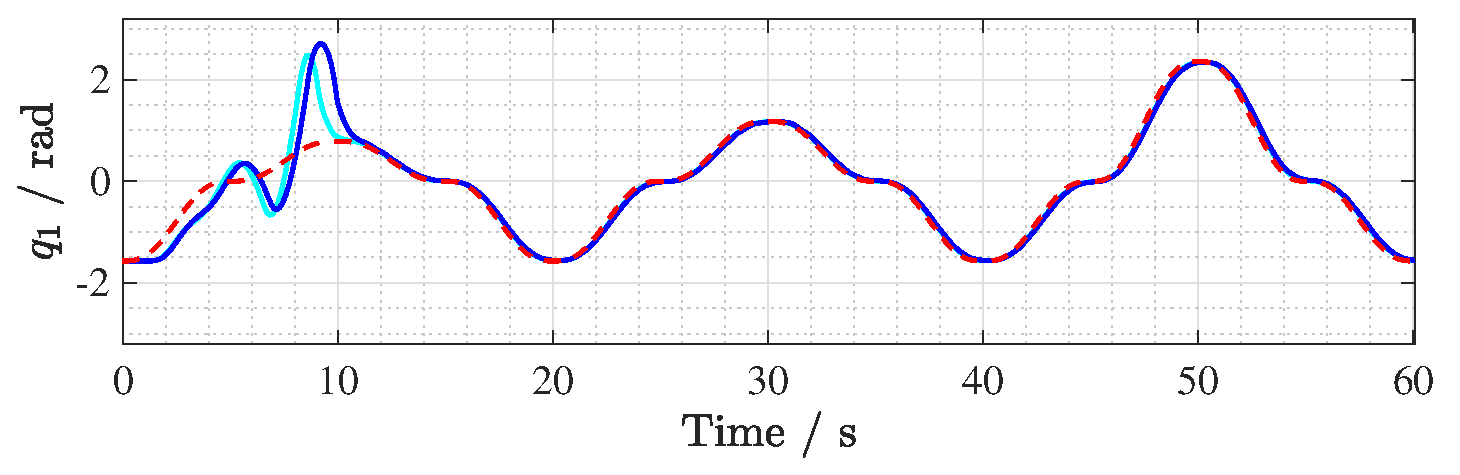
\includegraphics[width=\figSizeTwoCol\linewidth]
      {
        % fig/Fig1.pdf
        src/measurement/figures/compare/Fig1.eps
      }%
      \label{fig:ctrl:result:q1}}
    \hfill
    \subfloat[Tracking result of $2$\textsuperscript{nd} joint angle $q_2$.]{
      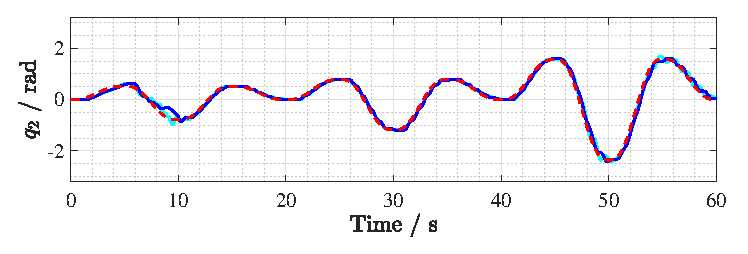
\includegraphics[width=\figSizeTwoCol\linewidth]
      {
        % src/measurement/figures/compare/Fig11.eps
        src/measurement/figures/compare/Fig2.eps
      }%
      \label{fig:ctrl:result:q2}}
    \vfill
      \subfloat[Control input $1$\textsuperscript{st} joint torque $\tau_1$.]{
        \includegraphics[width=\figSizeTwoCol\linewidth]
        {
            src/measurement/figures/compare/Fig3.eps
        }%
        \label{fig:ctrl:result:tau:1}}
    \hfill
      \subfloat[Control input $2$\textsuperscript{nd} joint torque $\tau_2$.]{
        \includegraphics[width=\figSizeTwoCol\linewidth]
        {
            src/measurement/figures/compare/Fig4.eps
        }%
        \label{fig:ctrl:result:tau:2}}
        \vfill
    \subfloat[Norm of control input (joint torque)$\rbu$.]{
        \includegraphics[width=\figSizeTwoCol\linewidth]
        {
            src/measurement/figures/compare/Fig5.eps
        }%
        \label{fig:ctrl:result:tau:norm}}
    \hfill
    \subfloat[Norm of DNN weights ${\estwth}_i$.]{
        % \includegraphics
        \includegraphics[width=\figSizeTwoCol\linewidth]
        {
            % fig/Fig7.pdf
            src/measurement/figures/compare/Fig7.eps
        }%
        \label{fig:ctrl:result:weight}}        
    \caption{
    Real-time implementation results of (C$_1$) \protect\colorLine{blue}{solid}, (C$_2$) \protect\colorLine{cyan}{solid}, (C$_3$) \protect\colorLine{gray}{solid}, (C$_4$) \protect\colorLine{magenta}{solid}, and desired trajectory $\qd$ \protect\colorLine{red}{dashed}.
  }
\label{fig:ctrl:result}
\end{figure*}

% ------------------------------------
% Norm of error in Episode 1: 
% C1 e1 ep1: 25.130
% C1 e2 ep1: 25.016
% C2 e1 ep1: 21.719
% C2 e2 ep1: 10.530
% C3 e1 ep1: 23.168
% C3 e2 ep1: 13.061
% C4 e1 ep1: 24.195
% C4 e2 ep1: 12.927
% Norm of error in Episode 2: 
% C1 e1 ep2: 7.066
% C1 e2 ep2: 2.198
% C2 e1 ep2: 8.021
% C2 e2 ep2: 2.435
% C3 e1 ep2: 8.408
% C3 e2 ep2: 3.554
% C4 e1 ep2: 19.721
% C4 e2 ep2: 4.256
% Improvement in Episode 2: 
% C1 e1: 0.719
% C1 e2: 0.912
% C2 e1: 0.631
% C2 e2: 0.769
% C3 e1: 0.637
% C3 e2: 0.728
% C4 e1: 0.185
% C4 e2: 0.671
% ------------------------------------

\begin{table}[!t]
    \renewcommand{\arraystretch}{1.3}
    \caption{Quantitative\,comparison\,of\,performances'\,$L_2$\,norm.}
    \centering
    \begin{tabular}{c c c c c}
    \hline
		& \multicolumn{4}{c}{\textbf{Episode 1}} \\
    \hline
	\hline 
		& (C$_1$) & (C$_2$) & (C$_3$) & (C$_4$) \\
	\hline
		$e_1\times10^{3}$ / rad & $25.130$ & $21.719$ & $23.168$ & $24.195$ \\ 
	\hline
        $e_2\times10^{3}$ / rad & $25.016$ & $10.530$ & $13.061$ & $12.927$ \\
	\hline
        & \multicolumn{4}{c}{\textbf{Episode 2}} \\
    \hline
    \hline
        & (C$_1$) & (C$_2$) & (C$_3$) & (C$_4$) \\
	\hline
    \multirow{2}{*}{$e_1\times10^{3}$ / rad} 
        & $7.066$ & $8.021$ & $8.408$ & $19.721$ \\
        & ($-71.6\%$) & ($-63.1\%$) & ($-63.7\%$) & ($-18.5\%$) \\
    \hline
    \multirow{2}{*}{$e_2\times10^{3}$ / rad} 
        & $2.198$ & $2.435$ & $3.554$ & $4.256$ \\
        & ($-88.4\%$) & ($-76.9\%$) & ($-72.8\%$) & ($-67.1\%$) \\
    \hline
    \end{tabular}
    \label{tab:sim:L2}
\end{table}

\subsection{Validation Results}

% ------------------------------------
% Tracking Performance
% ------------------------------------
\subsubsection{Tracking Performance}

The real-time implementation results are presented in Fig.~\ref{fig:ctrl:result}, and the quantitative comparison of tracking performance is summarized in Table~\ref{tab:sim:L2}.
Across the two episodes, all controllers improved their tracking performance. 
Specifically, the $L_2$-norm of $e_1$ was reduced by $71.6 \%$ for (C$_1$), $63.1 \%$ for (C$_2$), $63.7 \%$ for (C$_3$), and $18.5 \%$ for (C$_4$); while the $L_2$-norm of $e_2$ was reduced by $88.4 \%$, $76.9 \%$, $72.8 \%$, and $67.1 \%$, respectively.
Qualitatively, as illustrated in Fig.~\ref{fig:ctrl:result:q1} and Fig.~\ref{fig:ctrl:result:q2}, oscillations were suppressed during the second episode.
These results indicate that the DNNs in all controllers successfully learned the ideal control input $\rbu^*$ using the filtered tracking error $\fe$, despite $\rbu^*$ being completely unknown a priori.
Furthermore, the stable learning achieved under random weight initialization and no prior knowledge of the system, demonstrated the effectiveness of the proposed CONAC in enabling online learning capability.

Notably, in both episodes, all controllers failed to track the desired trajectory of $q_1$ during certain time intervals: from $17.5$ s to $19.9$ s in Episode $1$, and from $23.5$ s to $25.9$ s and from $29.5$ s to $31.9$ s in Episode $2$, as shown in Fig.~\ref{fig:ctrl:result:q1}.
This degradation in tracking performance is attributed to actuator saturation during those intervals, as observed in Fig.~\ref{fig:ctrl:result:tau:2} and Fig.~\ref{fig:ctrl:result:tau:norm}.

The tracking performance of CONAC with control input constraints—\ie (C$_1$) and (C$_2$)—outperformed the auxiliary system-based CONAC (C$_4$) in the second episode, as shown in Table~\ref{tab:sim:L2}.
This improvement is due to the fact that (C$_1$) and (C$_2$) were able to fully utilize the actuator's capabilities, whereas (C$_4$) was constrained by the auxiliary system's design, which limited the first joint actuator.
While (C$_3$) also showed better performance than (C$_4$), this was primarily because it did not consider input saturation and thus used more of the actuator's capacity.
However, since (C$_3$) did not handle the control input saturation, it generated excessively large control efforts to minimize the tracking error, even though these efforts could not be realized due to actuator limits, as shown in Fig.~\ref{fig:ctrl:result:tau:1}–\ref{fig:ctrl:result:tau:norm}.
In addition, the magnitude of saturation violations for (C$_3$) increased during each interval where input constraints were active.
Such large violations may lead to actuator damage or failure, posing a significant risk to the physical system.
Moreover, once the control saturation was released—typically due to a change in the desired trajectory—these large violations resulted in oscillatory behavior, as CONAC's weights had been adapted to produce excessively high control inputs, as shown in Fig.~\ref{fig:ctrl:result:tau:1}–\ref{fig:ctrl:result:tau:norm}.

% ------------------------------------
% Control Input Saturation
% ------------------------------------
\begin{figure}[t]
    \centering
    \subfloat[Control input $\tau$ locus in time interval from $29.4$ s to $31.9$ s.]{
    % \subfloat[Auxiliary states $\mv{\zeta}$ of CONAC-AUX.]{
        \includegraphics[width=\figSizeOneCol\linewidth]
        {
            src/measurement/figures/compare/Fig6.eps
        }%
        \label{fig:ctrl:result:scope:control}}
        \vfill
    \subfloat[Lagrange multipliers $\lambda_j,\forall j\in\mathcal{I}$ in time interval from $29.4$ s to $31.9$ s.]{
        \includegraphics[width=\figSizeOneCol\linewidth]
        {
            src/measurement/figures/compare/Fig8.eps
        }%
        \label{fig:ctrl:result:scope:beta}}
        \vfill
    \subfloat[Auxiliary states in time interval from $29.4$ s to $31.9$ s.]{
        \includegraphics[width=\figSizeOneCol\linewidth]
        {
            src/measurement/figures/compare/Fig9.eps
        }%
        \label{fig:ctrl:result:scope:aux}}
  \caption{
    Constraint handling process of (C$_1$) \protect\colorLine{blue}{solid}, (C$_2$) \protect\colorLine{cyan}{solid}, (C$_3$) \protect\colorLine{gray}{solid}, and (C$_4$) \protect\colorLine{magenta}{solid} in time interval from $29.4$ s to $31.9$ s.
  }
\label{fig:ctrl:result:scope}
\end{figure}

\begin{figure}[!t]
	\centering
	\includegraphics[width=0.7\linewidth]{
		src/figures/lambda_effect.drawio.pdf
		}
	\caption{
        The effect of the Lagrange multiplier $\lambda_{j}$ on the adaptation direction of $\widehat{\mv{\theta}}_2$ is illustrated. 
        The notations $(\cdot)'$ and $(\cdot)''$ denote two distinct cases corresponding to large and small values of the Lagrange multiplier, respectively, \ie $\lambda_{j}' > \lambda_{j}''$.
	}
	% \vspace{1mm}
	\label{fig:lambda_effect}
\end{figure}

\hfill

\subsubsection{Constraint Handling} \label{sec:sim:constraint}

In this section, the constraint handling capability of all controllers are investigated.
As shown in Fig.~\ref{fig:ctrl:result:tau:1}–\ref{fig:ctrl:result:tau:norm}, all controllers except (C$_3$) which did not consider the control input saturation, satisfied the control input saturation illustrated in Fig.~\ref{fig:robot:sat}.
For (C$_1$) and (C$_2$), the control input saturation was handled using corresponding input constraints in the constrained optimization framework and, for (C$_4$), the auxiliary system was utilized, as summarized in Table~\ref{table:controllers}.

To investigate the constraint handling process, the time interval from $29.4$ s to $31.9$ s was selected, during which the control input saturation was active for all controllers.
In Fig.~\ref{fig:ctrl:result:scope}, the control input locus, the Lagrange multipliers, and the auxiliary states are illustrated during this time interval.
The properties of the controllers can be observed in Fig.~\ref{fig:ctrl:result:scope:control}, where the control input locus of (C$_1$) and (C$_2$) fully explores the feasible domain of control input illustrated in Fig.~\ref{fig:robot:sat}, while (C$_3$) exceeds the input saturation limits, and (C$_4$) is limited in its first actuator input by the auxiliary system design.

% beta
The detail of the input constraint handling during the time interval from $29.4$ s to $31.9$ s, is now investigated.
In the cases of (C$_1$) and (C$_2$), as the input constraints $c_j$ were activated, the corresponding Lagrange multipliers $\lambda_j$ were generated dynamically, as shown in Fig.~\ref{fig:ctrl:result:scope:beta}.
These Lagrange multipliers directed the adaptation of the weights $\estwth_i,\ \forall i\in\{0,1,2\}$, to reduce violations of the constraints $c_j$, according to \eqref{eq:adap:th}.

% comparison; big, small beta
For more details, the growth effect of some convex input constraint's Lagrange multiplier $\lambda_j$ on the adaptation direction of $\estwth_2$ is illustrated in Fig.~\ref{fig:lambda_effect}, where two different magnitudes of $\lambda_j$ are considered. 
With this configuration, the difference between (C$_1$) and (C$_2$) can be investigated, as well, \ie large and small update rate $\beta_j$, since, for instance, (C$_1$) with large update rate $\beta_j$ leads to a larger Lagrange multiplier $\lambda_j$ than (C$_2$) with small update rate, see \eqref{eq:adap:lbd}.
Notably, under Assumptions \ref{assum:convex} and \ref{assum:LICQ}, the constraint $c_j$ is convex in the $\estwth_2$-space, see Lemma~\ref{lem:convex:angle}.

As illustrated in Fig.~\ref{fig:lambda_effect}, with large Lagrange multiplier $\lambda_j$, the adaptation direction of $\estwth_2$ is significantly influenced by the term $-\lambda_j\pptfrac{c_j}{\estwth_2}$ in \eqref{eq:adap:th}, which directs the weights toward satisfactory point of the constraint.
Hence, this results in a more aggressive adjustment of the weights leading to faster constraint satisfaction—but at the cost of oscillatory behavior in the learning process.
In Fig.~\ref{fig:ctrl:result:scope:control} and Fig.~\ref{fig:ctrl:result:scope:beta}, the earlier reasoning can be observed, where (C$_1$) with large update rate $\beta_j$ satisfied the input constraint $c_{\overline{\tau}_1}$ faster than (C$_2$) with repeatedly growing and resetting $\lambda_{\rbu}$.
In contrast, with small $\lambda_j$, the adaptation direction of $\estwth_2$ is less influenced, leading to a more conservative adjustment of the weights adaptation.
Consequently, the constraint satisfaction is achieved more smoothly, but potentially at the cost of slower satisfaction (convergence), as shown in Fig.~\ref{fig:ctrl:result:scope:control} and Fig.~\ref{fig:ctrl:result:scope:beta}.

% zeta
For (C$_4$), the auxiliary state $\zeta_1$ was generated in response to the control input saturation of the first link actuator $\tau_1$, as shown in Fig.~\ref{fig:ctrl:result:scope:aux}.
Since the weights were adapted to reduce both the filtered error $\fe$ and the auxiliary state $\mv{\zeta}$, the control input saturation was subsequently reduced, as evident in Fig.~\ref{fig:ctrl:result:scope:control}.
Once the saturation was resolved at approximately $31$ s (see Fig.~\ref{fig:ctrl:result:scope:control}), the auxiliary state $\zeta_1$ converged to zero due to the stable state matrix $\mm{A}_\zeta$ in the auxiliary system dynamics, given by $\ddtt\mv{\zeta} = \mm{A}_\zeta \mv{\zeta} + \mm{B}_\zeta \Delta\rbu$ with $\Delta\rbu=\mv{0}_{2\times1}$, as shown again in Fig.~\ref{fig:ctrl:result:scope:aux}.

\hfill 

Finally, the handling of the weight norm constraints $c_{\theta_i},\ \forall i\in\{0,1,2\}$, is investigated. 
Among all controllers, the weight norm constraint was only activated for the output layer weights $c_{\theta_2}$ in (C$_3$), as shown in Fig.~\ref{fig:ctrl:result:weight}. 
This is because the weights in (C$_1$), (C$_2$), and (C$_4$) were implicitly suppressed by the control input constraints, whereas (C$_3$) did not incorporate such constraints.
% , \ie by limiting the control input, the weight norms were also limited.
% \MSRY{필요하다면 왜 제어입력 제약하는게 가중치 제약도 되는지 추가 가능}
Furthermore, the constraints on the inner and hidden layer weights were never violated; that is, $\norm{\estwth_0}$ and $\norm{\estwth_1}$ consistently remained below their limits.
This is attributed to the fact that the backpropagated error was scaled by the gradient of the activation function, which is bounded between $-1$ and $1$; see \eqref{eq:NN:grad}.

Additional details on the constraint handling process are provided in Fig.~\ref{fig:ctrl:result:scope:beta}. 
Similar to the case of the control input constraints, the Lagrange multipliers $\lambda_{\theta_2}$ increased when $\estwth_2$ exceeded the prescribed norm constraint 
$\overline\theta_2$ at approximately $30.4$ s, as shown in Fig.~\ref{fig:ctrl:result:weight}, prompting an adjustment in the adaptation direction of $\estwth_2$ to mitigate the violation of the constraint $c_{\theta_2}$, as shown in Fig.~\ref{fig:ctrl:result:scope:beta}.

% In addition, it is worth noting that the control input constraints were repeatedly violated even after the constraint handling mechanisms were applied, as shown in Fig.~\ref{fig:ctrl:result:scope:control}. 
% This occurred because the controllers were implemented in discrete time with a relatively low sampling rate of $250$ Hz.

% ------------------------------------
% Karush-Kuhn-Tucker (KKT) conditions}
% ------------------------------------
\hfill

\subsubsection{Satisfaction of Karush-Kuhn-Tucker (KKT) conditions}

Since the proposed CONAC was implemented in discrete time, a direct demonstration of the KKT conditions at steady state is not straightforward. 
However, the near-constant values of the weights and Lagrange multipliers during constraint violation suggest an implicit satisfaction of the KKT conditions, as shown in Fig.~\ref{fig:ctrl:result:weight} and Fig.~\ref{fig:ctrl:result:scope:beta}.
Specifically, the Lagrange multipliers corresponding to active constraints were positive, while those associated with inactive constraints remained zero.

% reference 자체가 계속 움직이니까 엄밀하게는 steady state를 보장할 수 없습니다. rough 하게는 theta norm이 어느정도 수렴하므로 이 것을 기반으로 주장해볼 수도 있습니다. theta_dot이 평균적으로는 0에 가까운 것 같서요

% ------------------------------------
% Computational Time
% ------------------------------------
\hfill

\subsubsection{Effectiveness of CONAC in Real-time Applications}

The effectiveness of the proposed CONAC in real-time applications was evaluated by measuring the computational time using CPU clock ticks on the OpenCR1.0 board. 
As shown in Fig.~\ref{fig:ctrl:real:result:cmp:time}, the computational times of all controllers remained below $4$ ms, demonstrating that the proposed CONAC is suitable for real-time implementation at a sampling rate of $250$ Hz.

\begin{figure}[t]
    \centering
        \includegraphics[width=\figSizeOneCol\linewidth]
        {
            src/measurement/figures/compare/Fig10.eps
        }%
    \caption{
        Computational time of (C$_1$) \protect\colorLine{blue}{solid}, (C$_2$) \protect\colorLine{cyan}{solid}, (C$_3$) \protect\colorLine{gray}{solid}, and (C$_4$) \protect\colorLine{magenta}{solid}.
    }
    \label{fig:ctrl:real:result:cmp:time}
  \end{figure}

%  SECTION CONCLUSION ======================================
\section{Conclusion}\label{sec:conclusion}

This paper proposed a constrained optimization-based neuro-adaptive controller (CONAC) for \color{red}unkown\color{black} Euler-Lagrange systems, addressing both weight norm and input constraints through a rigorous optimization framework. 
The stability of the proposed CONAC was analyzed via Lyapunov theory, demonstrating bounded tracking and weight estimation errors under real-time adaptation.

The proposed CONAC effectively incorporated both convex input constraints and weight norm constraints, ensuring that actuator limitations and neural network weights remained within predefined bounds. 
By embedding these constraints into the optimization process, CONAC ensured convergence of the weights in accordance with the Karush-Kuhn-Tucker (KKT) conditions, thereby achieving both stability and optimality.

A real-time implementation validated the superior performance of CONAC compared to conventional methods. 
The proposed CONAC successfully handled complex input constraints while rigorously managing weight norms, resulting in improved tracking accuracy and stable performance without significant oscillations.

Future work may extend this approach to include constraints on both control inputs and system states, further enhancing the flexibility and robustness of neuro-adaptive control systems within constrained optimization frameworks.

%% The Appendices part is started with the command \appendix;
%% appendix sections are then done as normal sections
\appendix

\subsection{Input Constraint Candidates}\label{sec:appen:cstr} 

This section introduces potential input constraints that can be incorporated into the proposed CONAC framework.

\subsubsection{Input Bound Constraint}\label{sec:appen:cstr:input:bound}

Most physical systems are subject to control input limitations due to inherent electrical and mechanical constraints.
These are expressed as $\mv{c}_{\overline \tau}:= [c_{\overline \tau_i}]_{i\in\{1,\cdots,n\}}$ and $\mv{c}_{\underline\tau}:= [c_{\underline\tau_i}]_{i\in\{1,\cdots,n\}}$, where
\begin{equation}
    \begin{aligned}
        c_{\overline \tau_i}=\tau_{(i)} - {\tau_{\overline \tau_i}}
        ,
        \quad
        c_{\underline\tau_i}={\tau_{\underline\tau_i}}-\tau_{(i)}
        ,
    \end{aligned}
    \label{eq:cstr:input:bound}
\end{equation}
with $\tau_{\overline \tau_i}\in\R$ and $\tau_{\underline\tau_i}\in\R$ representing the maximum and minimum control input bounds, respectively.
The gradients of $\mv{c}_{\overline \tau}$ and $\mv{c}_{\underline\tau}$ with respect to $\estwth$ are given by
\begin{equation}
    \begin{aligned}
        \pptfrac{\mv c_{\overline \tau}}{\estwth}
        =& 
        \left[
            \pptfrac{c_{\overline \tau_i}}{\estwth}^\top
        \right]_{i\in\{1,\cdots,n\}}
        % \begin{bmatrix}
        %     \pptfrac{c_{\overline \tau_1}}{\estwth}^\top \\
        %     \vdots \\
        %     \pptfrac{c_{\overline \tau_n}}{\estwth}^\top
        % \end{bmatrix}
        = 
            +\pptfrac{\estNN}{\estwth}
            \\
        =&
        =
        +
        \begin{bmatrix}
            (\mm{I}_{l_{k+1}}\otimes \estact_{k}^\top)&
            \!\cdots\! &
            (
                \cdot
            )
        \end{bmatrix} 
        \in
        \mathbb R^{n\times \Xi}
        , 
        \\
        \pptfrac{\mv c_{\underline\tau}}{\estwth}         
        =
        & 
        \left[
            \pptfrac{c_{\underline\tau_i}}{\estwth}^\top
        \right]_{i\in\{1,\cdots,n\}}
        % \begin{bmatrix}
        %     \pptfrac{c_{\underline\tau_1}}{\estwth}^\top \\
        %     \vdots \\
        %     \pptfrac{c_{\underline\tau_n}}{\estwth}^\top
        % \end{bmatrix}
        = 
        -\pptfrac{\estNN}{\estwth}
        \\
        =&
        =
        -\begin{bmatrix}
            (\mm{I}_{l_{k+1}}\otimes \estact_{k}^\top)&
            % V_k^\top \phi_{k}' (I_{l_{k}}\otimes  \phi_{k-1}^\top)&
            \!\cdots\! &
            (
                \cdot
            )
        \end{bmatrix} 
        \in
        \mathbb R^{n\times \Xi}
        .
    \end{aligned}
    \label{eq:cstr:input:bound:grad}
\end{equation}

\subsubsection{Input Norm Constraint}\label{sec:appen:cstr:input:norm}

Consider the control input $\rbu$ as the torque corresponding to its generalized coordinate. 
Since torque is typically linearly proportional to current, actuators that share a common power source are often subject to total current limitations. This can be captured by the following inequality constraint: 
\begin{equation}
    c_{\rbu}
    =
    \tfrac{1}{2}\
    \left(
        \norm{
        \mv{\tau}
        }^2 
        -
        \overline\tau^2
    \right)
    ,
    \label{eq:cstr:input:norm}
\end{equation}
with $\overline\tau\in\R_{>0}$ denoting the maximum allowable control input magnitude. This input norm constraint is also commonly applied in current and torque control problems for electric motors \cite{Choi:2024aa}.
% The corresponding Lagrangian multiplier is $\lambda_{u_b}$. 
The gradients of $c_{\rbu}$ with respect to $\estwth$ are given by
\begin{equation}
    \pptfrac{\mv c_{\rbu}}{\estwth}
    \!=\! 
    \textstyle\sum_{i=1}^n \tau_{i} 
    \left(
        \myrow_i
        \left(
            \pptfrac{\estNN}{\estwth}
        \right)
    \right)^\top  
    \!=\! 
    {\pptfrac{\estNN}{\estwth}}^\top
    \mv{\tau}
    % \tau^\top (I_{l_{k+1}}\otimes \estNN_k^\top)
    \in \mathbb R^{\Xi}.
    \label{eq:cstr:input:norm:grad}
\end{equation}

\hfill

It should be noted that constraints \eqref{eq:cstr:input:bound} and \eqref{eq:cstr:input:norm} can be imposed simultaneously, as their gradients \eqref{eq:cstr:input:bound:grad} and \eqref{eq:cstr:input:norm:grad} are linearly independent, satisfying Assumption \ref{assum:LICQ}, \ie the LICQ condition.

\bibliographystyle{IEEEtran}
\bibliography{\template/refs}

\begin{IEEEbiography}[{
    \includegraphics[width=1in,height=1.25in,clip,keepaspectratio]{\template/people/msRyu.jpg}}]{Myeongseok Ryu}
    received the B.S. degree in Mechanical Engineering from Incheon National University, South Korea, in 2023, and the M.S. degree in Mechanical Engineering from GIST, South Korea, in 2025. 
    He is currently serving as a researcher at the Cho Chun Shik Graduate School of Mobility at KAIST, South Korea.
    His research interests include adaptive control, neural-networks, and constrained optimization.
\end{IEEEbiography}

\begin{IEEEbiography}[{
    \includegraphics[width=1in,height=1.25in,clip,keepaspectratio]{\template/people/dhHong.jpg}}]{Donghwa Hong}
    received his B.S. degree in Physics and Engineering Physics from Yonsei University, Wonju, South Korea, in 2023. He is currently pursuing the M.S. degree in Mechanical Engineering from GIST, Gwangju, South Korea.  
His research interests include robot control, neural-networks, and model identification. 
\end{IEEEbiography}

\begin{IEEEbiography}[{
    \includegraphics[width=1in,height=1.25in,clip,keepaspectratio]{\template/people/khChoi.jpg}}]{Kyunghwan Choi}
    received his B.S., M.S., and Ph.D. degrees in Mechanical Engineering from KAIST, Daejeon, South Korea, in 2014, 2016, and 2020, respectively. Following his Ph.D., he worked at the Center for Eco-Friendly \& Smart Vehicles at KAIST as a Postdoctoral Fellow and later as a Research Assistant Professor. In 2022, he joined GIST as an Assistant Professor in the Department of Mechanical and Robotics Engineering. Currently, he serves as an Assistant Professor at the Cho Chun Shik Graduate School of Mobility at KAIST, where he is also the Director of the Mobility Intelligence and Control Laboratory. His research focuses on optimal and learning-based control for connected, automated, and electrified vehicles (CAEVs).
\end{IEEEbiography}


\end{document}

